\documentclass[twocolumn,5p]{elsarticle}
\usepackage{tikz}
\def\firstcircle{(90:1.75cm) circle (2.5cm)}
\def\secondcircle{(210:1.75cm) circle (2.5cm)}
\def\thirdcircle{(330:1.75cm) circle (2.5cm)} 
\usepackage{comment}
\usepackage{framed,graphicx}
\usepackage{multirow}
\usepackage{rotating}
\usepackage{amsmath}
\usepackage{bigstrut}
\usepackage{color}
\usepackage{graphics} 
\usepackage{eqparbox}
\usepackage{graphics}
\usepackage{colortbl} 
%\usepackage{times}
\usepackage{mathptmx} \usepackage[scaled=.90]{helvet} \usepackage{courier}
\usepackage{balance}
\usepackage{picture}
\usepackage{algorithm}
\usepackage{algorithmicx}
\usepackage{algpseudocode}
\usepackage[export]{adjustbox}
\renewcommand{\footnotesize}{\scriptsize}
\definecolor{lightgray}{gray}{0.8}
\definecolor{darkgray}{gray}{0.6}
\definecolor{lavenderpink}{rgb}{0.98, 0.68, 0.82}
\definecolor{celadon}{rgb}{0.67, 0.88, 0.69}
\renewcommand{\algorithmicrequire}{\textbf{Input:}}
\renewcommand{\algorithmicensure}{\textbf{Output:}}
%%% graph
\newcommand{\crule}[3][darkgray]{\textcolor{#1}{\rule{#2}{#3}}}

\newcommand{\quart}[4]{\begin{picture}(80,4)%1
	{\color{black}\put(#3,2){\circle*{4}}\put(#1,2){\line(1,0){#2}}}\end{picture}}

\definecolor{Gray}{gray}{0.95}
\definecolor{LightGray}{gray}{0.975}

\newcommand{\wei}[1]{\textcolor{red}{Wei: #1}} 
\newcommand{\Menzies}[1]{\textcolor{red}{Dr.Menzies: #1}} 

%% timm tricks
\newcommand{\bi}{\begin{itemize}[leftmargin=0.4cm]}
	\newcommand{\ei}{\end{itemize}}
\newcommand{\be}{\begin{enumerate}}
	\newcommand{\ee}{\end{enumerate}}
\newcommand{\tion}[1]{\S\ref{sect:#1}}
\newcommand{\fig}[1]{Figure~\ref{fig:#1}}
\newcommand{\tab}[1]{Table~\ref{tab:#1}}
\newcommand{\eq}[1]{Equation~\ref{eq:#1}}


\usepackage[shortlabels]{enumitem}  
\usepackage{url}

\definecolor{Gray}{rgb}{0.88,1,1}
\definecolor{Gray}{gray}{0.85}
% \usepackage[svgnames]{xcolor}
\usepackage[framed]{ntheorem}
\usepackage{framed}
\usepackage{tikz}
\usetikzlibrary{shadows}
%\newtheorem{Lesson}{Lesson}
\theoremclass{Lesson}
\theoremstyle{break}

% inner sep=10pt,
\tikzstyle{thmbox} = [rectangle, rounded corners, draw=black,
fill=Gray!40,  drop shadow={fill=black, opacity=1}]
\newcommand\thmbox[1]{%
	\noindent\begin{tikzpicture}%
	\node [thmbox] (box){%
		\begin{minipage}{.94\textwidth}%    
		\vspace{-2mm}#1\vspace{-3mm}%
		\end{minipage}%
	};%
	\end{tikzpicture}}

\let\theoremframecommand\thmbox
\newshadedtheorem{lesson}{Result}



\begin{document}
	
	\begin{frontmatter}
		
		% \title{How to Discourage Useless Refactorings}
		\title{Toward Intelligent Refactoring Recommendations}
		
		\author{Rahul Krishna\corref{cor1}\textsuperscript{a,}}
		\ead{rkrish11@ncsu.edu}
		\author{Tim Menzies\corref{cor1}\textsuperscript{a,}}
		\ead{tim.menzies@gmail.com}
		\author{Lucas Layman\textsuperscript{b}}
		\ead{ llayman@cese.fraunhofer.org }
		\cortext[cor1]{Corresponding author: Tel:+1-919-396-4143(Rahul)}
		\address{\textsuperscript{a}Department of Computer Science, North Carolina State University, Raleigh, NC, USA\\
			\textsuperscript{b}Fraunhofer CESE, College Park, USA}
		\pagenumbering{arabic}
		
		\begin{abstract} 
			{\bf Context: } 
			Developers use bad code smells to guide refactoring.
			Yet developers, text books, tools, and researchers disagree on which bad smells are important.
			%Many bad smell detectors recommend refactoring when static code measure
			%cross some threshold boundary. 
			%%However, it is unclear at what threshold values smell-related metrics
			%should trigger code improvement or preventative maintenance.  
			
			\noindent 
			{\bf Objective:} To evaluate the likelihood that a refactoring to address bad code smells will yield improvement in the defect-proneness of the code.
			
			\noindent
			{\bf Method: } We introduce XTREE, a tool that analyzes a historical log of defects seen previously in the code and generates a set of useful\footnote{Need to define useful in precise terms} code changes.
			Any bad smell that requires changes outside of that set can be deprioritized (since there is no historical evidence that the bad smell causes any problems).
			
			\noindent
			{\bf Evaluation: } We evaluate XTREE's recommendations for bad smell improvement against recommendations from previous work (Shatnawi, Alves, and Borges) using multiple data sets of code metrics and defect counts.  
			
			\noindent
			{\bf Results: }Code modules that are changed in response to XTREE's recommendations contain significantly fewer defects than recommendations in previous studies. Further, XTREE endorses changes to very few code metrics, and those bad smell recommendations (learned from previous studies) are not universal to all  software projects.
			
			\noindent
			{\bf Conclusion: }
			Before undertaking a refactoring based on a bad smell report,
			use a tool like XTREE to check and ignore any refactorings   that  are useless; i.e. which lacks evidence
			in the historical record  that it is useful to make that change.
			Note that this use case applies to both manual refactorings proposed by developers
			as well as refactoring  conducted by automatic methods.
			This recommendation assumes that there is an historical record.
			If none exists, then the results of this paper could be use used as a guide (see our
			Table~8). 
			
			
		\end{abstract}
	\end{frontmatter}
	\pagenumbering{arabic} %XXX delete before submission
	
	\vspace{1mm}
	\noindent
	{\bf Keywords:} Bad smells,
	performance prediction,  decision trees 
	
	
	
	
	\section{Introduction}
	
	According to   Fowler ~\cite{fowler99}, bad smells (a.k.a. code smells)
	are ``a surface indication that usually corresponds to a deeper problem''.
	Fowler strongly recommends   removing   code smells   by
	\begin{quote}
		``...applying a series of small behavior-preserving transformations, each 
		of which seem ``too small to be worth doing''. 
		The  effect of   these \underline{refactoring} transformations is quite significant. By doing them in small steps you reduce the risk 
		of introducing errors''.
	\end{quote}
	
	Bad smells are a widely used technique for evaluating code. While the original bad small concept was largely subjective [REF], researchers including Marinescu [REF] and others has provided formal definitions of ``bad smells'' in terms of static code attributes such size, complexity, coupling, and other metrics. Consequently, code smells are captured by popular static analysis tools such as PMD [REF], CheckStyle [REF], FindBugs [REF], and SonarQube [REF], although not always explicitly labeled as such. 
	
	Refactoring bad smells from code is generally accepted as a recommended practice, but refactoring by definition does not change the external functionality of the system and thus may have no perceived value. For example, this paper began when a Washington-based software company shared one of their management challenges with us: their  releases are delayed by developers spending  much time removing bad smells within their code. 
	%This management team wanted some way to check if all that activity was useful. 
	Kim et al.\cite{kim2012field} surveyed developers at Microsoft and found that refactoring incurs significant cost and risks. A Google search on the terms ``refactoring cost'' yields numerous threads on StackOverlfow from developers asking how to justify refactoring and when the costs of refactoring outweight its benefits. 
	
	
	% As of  early 2016, the ACM Digital Library reports 
	% the Fowler text of {\em Refactoring} has 6434 references~\cite{fowler99}. A search  on \texttt{``bad smell'' programming 
	% where proceedings=ICSE} in the ACM Digital Library finds 1,748 papers since 2006.
	% Hence it is important to understand the value of
	% this popular topic.  
	% Valuable development resources may be wasted on bad smells that are ``bad''; i.e. 
	%  irrelevant or misleading
	% for some particular project.
	
	% In our experience, programmers can use the SE literature to justify extensive, perhaps even excessive, refactoring efforts.
	% For example, this paper began when a Washington-based software company shared
	% one of their management challenges with us: their  releases are delayed by developers spending  much time removing bad smells within their code. This management team wanted some way to check if all that activity was useful.
	
	% In addition to tools that capture bad smells such as FindBugs and SonarQube, a multitude of tools have been proposed to support refactoring (e.g., \cite{ge2014manual,lee2013drag,foster2012witchdoctor,ge2012reconciling}). Note that these managers are {\em not} asking for better
	% automatic refactoring
	% tool support. 
	% Their human programmers are refactoring
	% code all the time, perhaps too much so.
	% Hence, the management goal
	The challenge is to encourage refactorings that result in perceivable benefits (such as reduced defect proneness or lower maintenance costs) and avoid refactorings with no demonstrable benefit and thus waste effort.
	
	This paper describes one approach to evaluate whether refactorings that change the structure of code are likely to have a perceivable benefit by evaluating:
	\bi
	\item If there is no evidence in the historical record that changing ``X'' is useful;
	\item Then discourage developers from doing ``X''.
	\ei
	We use data mining to generate two oracles: a {\em primary
		change oracle} and a {\em secondary verification oracle}.
	By combining these two oracles,
	we can generate and validate useful
	changes to code modules. We focus on ``bad smells'' indicated by code metrics such as size and complexity as captured in popular tools such as SonarQube [REF] and Klocwerk [REF].
	
	In this paper, we use 
	the XTREE cluster delta algorithm as the {\em primary change  oracle}.
	XTREE 
	explores the historical record of a project to find clusters of module.
	It then proposes a ``minimal'' set of changes $\Delta$ that can move a software module $M$ from a defective cluster $C_0$ to another with fewer defects $C_1$ (so $\Delta$
	is some subset of $C_1 - C_0$). % To define ``minimal'', XTREE uses an entropy measure.
	
	As to 
	the {\em secondary verification oracle}, this  checks if the primary oracle is proposing
	sensible changes. For this purpose we use Random Forest~\cite{breiman2001random}, augmented with SMOTE (synthetic  minority over-sampling technique~\cite{chawla2002smote}).
	In our framework,  learning
	the secondary oracle is   a {\em separate} task from that of learning the primary
	oracle. This  ensures that the verification oracle offers an independent
	opinion on the value of the proposed changes.
	
	When these oracles were applied to defect data from
	open source object-oriented software systems, we discovered a {\em conjunctive fallacy}
	in the bad smell literature~\cite{erni96,bender99,Shatnawi10,Alves2010,hermans15}.
	A common heuristic is to recommend refactoring of ``bad'' code
	to make it ``better'' as follows: for all static code measures that exceed some threshold, make changes such that the thresholds are no longer exceeded. That is:
	\begin{equation}\label{eq:df}
		\scriptstyle
		\begin{array}{rl}
			\mathit{bad}    & = \left(a_1 > t_1 \right) \bigvee \left(a_2 > t_2\right) \bigvee    ...                             \\
			\mathit{better} & = \neg\;\mathit{bad} = \left(a_1 \le t_1 \right) \bigwedge \left(a_2 \le t_2\right)  \bigwedge  ... 
		\end{array}
	\end{equation}
	We say that the above definition of ``better'' is a conjunctive fallacy
	since it assumes that the best way to improve code is to decreases multiple code attribute measures below $t_i$ in order
	to remove the ``bad'' smells. In reality, there exists an intricate set of associations between static code measures
	such that {\em decreasing}  $a_i$ necessitates {\em increasing} $a_j$.
	It is easy to see why this is so.
	A requirement for  refactoring is that the new code supports the same functionality
	as before. If we pull code out of a function (since that function has grown too
	large), {\em that functionality has to go somewhere else}. What we see in XTREE's change
	recommendation is that if we decrease a module's lines of code  then in the refactored
	code, the functionality is achieved via a communication between several different parts
	of the system. That is, {\em decreasing} the lines of code metric within a module {\em increases}
	that module's coupling metrics.
	
	\subsection{Structure of this Paper}
	
	This paper  claims that (a)~XTREE is a  better way than \eq{df}  to define useful changes to software and (b)~those changes are useful for recognizing   superfluous refactorings since they usually refer to a very 
	small subset of the static code measures (which allows us to rule out refactorings based on any of the omitted
	static code measures). 
	In support of these claims, 
	the rest of this paper is structured as follows. In Section~2, we offer some background on bad smells. In Section~3, 
	different methods are presented for determining when code does/does not have bad smell. One of those methods
	will be XTREE while the others will come from other researchers. Section~4
	defines an assessment method that checks which of these methods is most useful. The results from that assessment 
	are presented in Section~5. Those results will answer five research questions.
	
	{\bf  RQ1: Effectiveness}\footnote{test}: According to the verification oracle, which of the methods  defined in Section~3 is the best  change oracle for identifying what and how
	code modules should be changed? To answer this question, we used data from five OO Java projects
	(Ivy, Lucene, Ant, Poi, Jedit). It was found that:
	\begin{lesson}
		XTREE is the most accurate oracle on how to change code modules in order to reduce defects.
	\end{lesson}
	
	{\bf RQ2: Succinctness}: Our goal is to critique and, possibly,
	ignore irrelevant bad smell detectors.  If those changes are minimal (i.e. affect fewest attributes) then those changes
	will be easiest to apply and monitor. Hence, we ask, which of the Section~3 methods recommended changes to the fewest
	code attributes?
	\begin{lesson}
		Of all the code change oracles studied here, XTREE recommends the fewest number of changes to static code measures.
	\end{lesson}
	
	{\bf RQ3: Stopping}: Our advice to managers is to discourage refactoring based on changes that lack
	historical evidence of being effective. How effective is XTREE at offering such ``stopping points'' (i.e. clear guidance on what {\em not} to do)??
	\begin{lesson}
		In  any  project,  XTREE's  recommended  changes  only  mentions one to four 
		of the  static code attributes.  Any bad smell defined in terms of the remaining 19 to 16 code attributes (i.e. most of them)
		would hence be deprecated.
	\end{lesson}
	
	{\bf RQ4: Stability}: Across different projects, how variable are the changes recommended by our best change oracle?
	\begin{lesson}
		The direction of change recommended by XTREE is  very stable across repeated runs of the program 
	\end{lesson} 
	
	{\bf RQ5: Conjunctive Fallacy}:  
	Is it always  useful  to aplly \eq{df}; i.e. make code better by   reducing the values of  multiple code attributes? We find that:
	\begin{lesson}
		XTREE usually recommends reducing lines of code (size of the modules).
		That said,  XTREE often recommends {\em increasing} the values of other static code attributes.
	\end{lesson} 
	Note that {\bf RQ3, RQ4, RQ5} 
	confirms the intuitions
	of the project managers that prompted this investigation:
	\bi
	\item
	Yes,  indeed, their programmers
	were wasting time on   performing refactorings  that  decreased multiple measures when, in fact,
	they should be trying to {\em decrease} some measures while {\em increasing} others.
	\item
	Across all studied projects, XTREE found that  around one-fifth  
	of the measures were usually found within  change recommendations. That is, it is 80\% likely that
	that refactoring based on reducing any one measurement picked at random will be useful.
	\ei
	Consequently, we  recommend the following use case for  XTREE:
	\bi
	\item Before doing  refactoring based on a bad smell report...
	\item ...check and discourage any refactoring   for which there is no proof
	in the historical record that the change improves the code.
	\ei
	This use case described  applies to both manual refactorings proposed by developers
	as well as refactoring conducted by automatic methods~\cite{mkaouer2015many}. That is, XTREE could optimize automatic
	code refactoring by discouraging refactorings for useless goals.
	
	
	
	\subsection{ Threats to Validity}
	
	The results of this paper are biased by out choice of refactoring goal (reducing defects) and our choice
	of measures collected from software project (OO measures such as
	depth of inheritance, number of child classes, etc).
	
	That said, it should be possible extend the methods of this paper to other kinds of goals (e.g. maintainability, reliability, security,
	or the knowledge sharing measures favoured by Bosu and Carver~\cite{bosu13}) and other kinds of inputs (e.g. the process measures favored by Rahman, Devanbu et al.\cite{Rahman2013})  as follows:
	\bi
	\item Find a data source for the other measures of interest;
	\item Implement another secondary verification oracle that can assess maintainability, reliability, security, etc;
	\item Implement a better primary verification oracle that can do ``better'' that XTREE at finding changes (where ``better'' is defined in terms 
	of the opinions of the verification oracle).
	\ei
	To assist other researchers exploring these points, we offer a full replication package for this study at  https://github.com/ai-se/XTREE\_IST.
	
	The results of this paper are also specific to the data sets explored here.
	Such sampling bias threatens any data mining experiment; i.e., what matters
	{\em there} may not be true {\em here}. For example, the data sets used here comes from a survey of
	open source JAVA projects from Jureczko et al.~\cite{jureczko10}. Any biases in their selection procedures
	threaten the validity of these results. 
	
	That said,
	the best we can do is define our methods and publicize our data and code so that other researchers can
	try to repeat our results and, perhaps, point out a previously unknown bias
	in our analysis. Hopefully, other researchers will emulate our methods in
	order to repeat, refute, or improve our results. 
	
	The recommendation to management, shown on page one of this paper,  was to discourage developers doing ``X'' if there was no historical evidence that ``X'' was useful. 
	This recommendation assumes that such an  historical record can be accessed. If not,  then the results of this paper could be use used as a guide (see our Table 8). Alternatively, some form of transfer learning~\cite{Nam15,Jing15,krishna16} could be used to import data from another project (but more research would be required to test the validity of combing tools like XTREEs with transfer learning). 
	
	
	
	
	\subsection{Relationship to Prior Work }
	A four page preliminary report on the XTREE system~\cite{krishna2015actionable} has been presented previously\footnote{https://goo.gl/2In3Lr}. That short report offered case studies on only two  of
	the five data sets studied here. Also, that prior work had:
	\bi
	\item
	no comparison to any baseline
	method from other researchers, whereas this paper compares XTREE's recommendations
	with those found by researchers exploring bad smells.
	\item
	no {\em secondary verification oracle}, i.e. no way to check if XTREE's recommended changes were sensible.
	\ei
	Further, of this entire paper, the only sections containing material
	found in prior papers is 3.2.1, 3.2.2 as well as two-fifths of the results in \fig{jur}. 
	
	
	
	\section{Why Not Just Ask Developers to Rank Bad Smells?}\label{sect:prelim}
	
	Why build tools like XTREE to  critique proposed developer actions?
	Our answer, documented in this section, is that (1)~SE literature is not clear which bad smells are ignorable or  high priority and must be resolved.
	Also, (2)~developers themselves are unclear on what bad smells are most important to fix.
	
	
	Much research endorses them to guide
	code improvement (e.g., refactoring or preventative maintenance). A recent literature review by Tufano et al.~\cite{Tufano2015}  
	lists dozens of papers on smell detection and repair tools. 
	Yet
	other papers cast doubt on the value of bad smells
	as triggers for code improvement~\cite{Mantyla2004,Yamashita2013,Sjoberg2013}. 
	As we show in this paper,  
	tools, text books, and developers disagree on what bad smells
	are important enough to hunt down and eliminate. Our findings
	are consistent with other research suggesting that universal bad
	smells that ignore project context are not useful to guide refactoring~\cite{Mantyla2004,Yamashita2013,Sjoberg2013}.
	
	If the SE literature is contradictory, why not ignore it and use domain experts (software engineers) to decide
	what bad smells to fix? We do not recommend this since developer {\em cognitive biases} can mislead them to
	assert that some things are important and relevant when they are not. 
	A widespread malaise in software engineering is that
	beliefs about software are rarely revised and hence may be
	inaccurate and 
	misleading~\cite{passos11,jorgensen09,mei15,me16phase,prem16}. Software developers may have strong views on many issues, including bad smells, but those views may be wrong for the current
	project.
	Software engineering is not the only field with this problem.
	For example, the medical profession applies many practices based on studies that have been disproved (a recent article in the Mayo Clinic Proceedings~\cite{prasad13} found 146 medical practices based on studies in year i, but which were reversed by subsequent trials within years i + 10). Even when the evidence for or against a treatment or intervention is clear, medical providers and patients may not accept it~\cite{aschwanden10}. Aschwanden warns that {\em cognitive biases} such as confirmation bias (the tendency to look for evidence that supports what you already know and to ignore the rest) influence how we process information~\cite{aschwanden15}.
	
	As in medicine, so too in software engineering.
	According to Passos et al.~\cite{passos11},  developers often  assume that the lessons they learn from a few past projects are general to all their future projects. They comment ``past experiences were taken into account without much consideration for their context''~\cite{passos11}.  J{\o}rgensen \& Gruschke~\cite{jorgensen09} offer a similar warning. They report that the supposed software engineering ``gurus'' rarely use lessons from past projects to improve their future reasoning and that such poor past advice can be detrimental to new projects.~\cite{jorgensen09}. Other studies have shown some widely-held views are   now questionable given new evidence:
	
	\bi
	% COMMENT FROM LL: This bullet is weak. Maybe goto isn't used in an unrestricted manner because of Djikstra's warning.
	% \item
	% Nagappan et al. analyzed~\cite{mei15} 
	% how   {\tt goto}  was used  in 11,000 Github repositories. 
	% They found that developers
	% rarely used {\tt goto} in the unrestricted manner that alarmed Dijkstra in his  1968
	% memo ``Go to statement considered harmful''~\cite{Dijkstra68}.
	\item
	In other work~\cite{me16phase} with the Software Engineering Institute (SEI), we have revisited
	the ``phase delay'' truism that {\em the cost of fixing an error dramatically increases the longer it is in the system}. 
	We found no evidence for such large   phase delay effect in modern
	software (in 171 software projects shepherded
	by the SEI, 2006-2014) possibly since it has been  heavily mitigated by $21^{st}$ century software development languages, tools and development practices. 
	Whatever the reason, the main point  is that phase delay is a widely
	held belief, despite little recent evidence to support it.
	\item
	Devanbu et al. examined responses from 564 Microsoft software developers from around
	the world, they found that  ``(a)~programmers do indeed have very
	strong beliefs on certain topics; (b)~their beliefs are primarily formed
	based on personal experience, rather than on findings in empirical
	research; (c)~beliefs can vary with each project, but do not necessarily
	correspond with actual evidence in that project''~\cite{prem16}.
	\ei
	Devanbu et al. further  comment that ``programmers give personal experience
	as the strongest influence in forming their opinions''. This is a troubling
	result, especially given the above comments from Passos and  J{\o}rgensen et al.~\cite{passos11,jorgensen09} about how quickly practitioners form, freeze, and rarely revist those opinions.
	
	
	
	\def\checkmark{\tikz\fill[scale=0.4](0,.35) -- (.25,0) -- (1,.7) -- (.25,.15) -- cycle;} 
\begin{figure}[!t] 
\scriptsize
\centering
\begin{tabular}{r|c|c|c|c} 


\begin{turn}{75}Fowler'99~\cite{fowler99} and~\cite{Kerievsky2005}\end{turn} &\begin{turn}{75} Lanza'06~\cite{Lanza2006}\end{turn} & \begin{turn}{75}SonarQube~\cite{sq15} \end{turn} &  \begin{turn}{75}Yamashita'13\cite{Yamashita2013} \end{turn}& \begin{turn}{75} Developer Survey 2015\end{turn}\\\hline
  Alt. Classes with Diff. Interfaces & & & & \\
  Combinatorial Explosion~\cite{Kerievsky2005} & & &  & \\
  Comments & & & 11 & VL\\
  Conditional Complexity~\cite{Kerievsky2005} & & & 14  & ?\\
  Data Class & \checkmark & &  &\\
  Data Clumps &  &  &  &\\
  Divergent Change & & &  & \\
  Duplicated Code & \checkmark & \checkmark & 1  & VH\\
  Feature Envy & \checkmark & & 8  &\\
  
  Inappropriate Intimacy & & \checkmark &  & L\\
  Indecent Exposure~\cite{Kerievsky2005} & & &  & ?\\
  Incomplete Library Class & & &  &\\
  Large Class & \checkmark & \checkmark & 4  & VH\\
  Lazy Class/Freeloader & & \checkmark & 7  &\\
  Long Method & \checkmark& \checkmark & 2  & VH\\
  Long Parameter List &  & \checkmark & 9  & L \\
  
  Message Chains & & &  & H\\
  Middle Man & &  &  &\\
  Oddball Solution~\cite{Kerievsky2005} & & &  & \\
  Parallel Inheritance Hierarchies & & &  &\\
  Primitive Obsession &  & &  &\\
  
  Refused Bequest & \checkmark & \checkmark &  & \\ 
  Shotgun Surgery & \checkmark& &  & \\
  Solution Sprawl~\cite{Kerievsky2005} & & &  &\\
  Speculative Generality & & &  & L\\
  Switch Statements &  & &  & L\\
  Temporary Field & & \checkmark &  & ?\\
  \end{tabular}
%   \multicolumn{5}{l}{} \\
%   \multicolumn{5}{l}{\textsuperscript{\textdagger} + Exact rule, - Possibly related rule} \\
%     \multicolumn{5}{l}{\textsuperscript{\textdaggerdbl} + is included in list} \\
%     \multicolumn{5}{l}{\textsuperscript{\textexclamdown} VH: Very High, H: High, L: Low, VL: Very Low, ?: Still investigating} \\
%   \multicolumn{5}{l}{\textsuperscript{*} Computation is based on more than simple metrics.} \\

\caption{Bad   smells from different sources.  Check marks (\protect\checkmark) denote   a bad smell was mentioned.
Numbers or symbolic labels (e.g. "VH") denote  a priorization comment (and
``?'' indicates lack of consensus). Empty cells
denote some bad smell listed in column one that was not found relevant
in other studies.
Note: there are many blank cells.}
\label{fig:smells}
\end{figure}
	
	If the above remarks hold true for bad smells, then we would expect
	to see much disagreement on which bad smells are important and relevant
	to  a particular project. This is indeed the case.
	The first column of \fig{smells} 
	lists  commonly mentioned bad smells and comes from Fowler's 1999 text~\cite{fowler99} and a subsequent 2005 text by Kerievsky that is widely cited~\cite{Kerievsky2005}.
	The other
	columns show data from other studies on which bad smells matter most.
	The columns marked as Lanza'06 and Yamashita'13 are from peer reviewed literature. The column maked SonarQube is a popular open source
	code assessment tool that includes detectors for six of the bad smells
	in column one. 
	The {\em developer survey} (in the right-hand-side column) shows the results of an hour-long whiteboard sessions with a group of 12 developers from a Washington
	D.C. web tools development company. Participants
	worked in a round robin manner to rank the bad smells they thought were
	important (and any disagreements were discussed with the whole group).
	Amongst the group, there was  some
	consensus on  the priority of which bad smells to fix
	(see the annotations VH=very high,
	H=high, L=low, VL=very low, and ``?''= no consensus).  
	
	
	
	\begin{figure*}[t!]
	\renewcommand{\baselinestretch}{0.8}\begin{center}
		{\scriptsize
			\begin{tabular}{c|l|p{4.7in}}
				amc & average method complexity & e.g. number of JAVA byte codes\\\hline
				avg\, cc & average McCabe & average McCabe's cyclomatic complexity seen
				in class\\\hline
				ca & afferent couplings & how many other classes use the specific
				class. \\\hline
				class. \\\hline
				cam & cohesion amongst classes & summation of number of different
				types of method parameters in every method divided by a multiplication
				of number of different method parameter types in whole class and
				number of methods. \\\hline
				cbm &coupling between methods &  total number of new/redefined methods
				to which all the inherited methods are coupled\\\hline
				cbo & coupling between objects & increased when the methods of one
				class access services of another.\\\hline
				ce & efferent couplings & how many other classes is used by the
				specific class. \\\hline
				dam & data access & ratio of the number of private (protected)
				attributes to the total number of attributes\\\hline
				dit & depth of inheritance tree &\\\hline
				ic & inheritance coupling &  number of parent classes to which a given
				class is coupled (includes counts of methods and variables inherited)
				\\\hline
				lcom & lack of cohesion in methods &number of pairs of methods that do
				not share a reference to an case variable.\\\hline
				locm3 & another lack of cohesion measure & if $m,a$ are  the number of
				$methods,attributes$
				in a class number and $\mu(a)$  is the number of methods accessing an
				attribute, 
				then
				$lcom3=((\frac{1}{a} \sum, j^a \mu(a, j)) - m)/ (1-m)$.
				\\\hline
				loc & lines of code &\\\hline
				max\, cc & maximum McCabe & maximum McCabe's cyclomatic complexity seen
				in class\\\hline
				mfa & functional abstraction & number of methods inherited by a class
				plus number of methods accessible by member methods of the
				class\\\hline
				moa &  aggregation &  count of the number of data declarations (class
				fields) whose types are user defined classes\\\hline
				noc &  number of children &\\\hline
				npm & number of public methods & \\\hline
				rfc & response for a class &number of  methods invoked in response to
				a message to the object.\\\hline
				wmc & weighted methods per class &\\\hline
				\rowcolor{lightgray}
				nDefects & raw defect counts & Numeric: number of defects found in post-release bug-tracking systems.\\
				\rowcolor{lightgray}
				defect & defects present? & Boolean: if {\em nDefects} $>0$ then {\em true} else {\em false}
			\end{tabular}
		}
	\end{center}
	\caption{OO code metrics used for all studies in this paper.
	   Last lines, shown in \textcolor{gray} denote the dependent variables.}\label{fig:ck}
\end{figure*}
	
	A  blank cell in \fig{smells}
	indicates where   other work has chosen to ignore
	one of the bad smells in column one. 
	Note that most of the cells are blank, and that the studies ignore the majority of the Fowler bad smells.
	SonarQube has no detectors for many of the column one bad smells.
	Also, nearly half the Yamashita list of bad smells
	does not appear in the Fowler and Kerievsky list. The eight numbers
	in the  Yamashita'13 column show the rankings for the bad smells 
	that overlap with Fowler and Kerievsky; Yamashita also discussed other smells not covered in Fowler'99.
	
	
	Two of the studies in \fig{smells} offers some comments on the relative importance
	of the different bad smells in the Yamashita'13 study and the developer study. Three of the bad smells listed in the top half of the Yamashita'13 rankings also score very high in the developer survey. Those three were {\em duplicated code, large class}, 
	and {\em long method}. 
	Note that this agreement also means that the
	Yamashita'13 study and the developer survey   
	believe
	that very few  code smells are   high priority issues
	requiring refactoring. 
	
	In summary, just because one developer strongly believes in the importance of a bad smells does not mean that belief transfers to other developers or projects.
	Developers can be clever, but their thinking can also be distorted
	by cognitive biases.
	Hence, as shown in \fig{smells}, developers, text books, and tools 
	can disagree on which bad smells are important.
	Special tools are needed to assess their beliefs, for example, their beliefs in
	bad smells.  
	
	
	\section{Learning Bad Smell Thresholds}\label{sect:bst}
	
	Having made the case for automatic support for assessing bad smells,
	this section reviews different ways for building those tools (one of those tools,
	XTREE, will be our recommended {\em primary change oracle}).
	Later in this paper, we will offer  a {\em secondary verification oracle}
	that checks the effectiveness of the changes proposed by XTREE.
	
	The SE literature offers two ways of learning bad smell thresholds.
	One approach relies on 
	{\em outlier statistics}~\cite{erni96,bender99}. This approach
	has been used   by Shatnawi~\cite{Shatnawi10}, Alvenes et al.~\cite{Alves2010}
	and Hermans et al.~\cite{hermans15}.
	Another approach is 
	based on {\em cluster deltas} that we developed
	for   Centroid Deltas~\cite{me12c} and 
	use here for XTREE. 
	These two approaches are discussed below. 
	
	\subsection{Outlier Statistics}
	
	The outlier approach assume that unusually large measurements indicate risk-prone code.
	Hence, they generate one bad smell threshold for any metric
	with such an ``unusually large'' measurement. 
	The literature lists several ways to define ``unusually large''.
	
	\begin{figure*}[t!]
~\hrule~
\begin{minipage}{.53\linewidth}
\small
 \begin{tabular}{p{0.95\linewidth}} 
 On the right-hand-side is a tree
 generated by iterative dichomization. 
 This tree can be read like a nested if-then-else statement; e.g.
 \begin{itemize}
     \item Lines 3 and 8 show two branches for lines of code (denoted here as {\em `\$loc}) below 698 and above 698.
     \item Any line with a colon ":" character shows  a  leaf  of  this  nesting.   For  example,  if  some  new  code module is passed down this tree and falls to the line marked in \textcolor{orange}{{\bf orange}},  the colon on that line indicates a prediction that this module has a 100\% chance of being defective. 
     \end{itemize}
Using this tree,
 XTREE looks for a nearby branch that has a lower chance of being defective. Finding the \textcolor{green}{{ green}} desired  branch,  XTREE reports a bad smell threshold for that module that is the delta between the \textcolor{orange}{{\bf orange}}  current branch  and   \textcolor{green}{{ green}} designed branch.
 In this case, that threshold relates to:
 \begin{itemize}
     \item Lines of code and comments ({\em lcom}) 
     \item The cohesion between classes ({\em cam}) which measures similarity of parameter lists to assess the relatedness amongst class   methods.
     \end{itemize}\\ 
 \end{tabular}
 \end{minipage}~~~~
 \begin{minipage}{.45\linewidth}
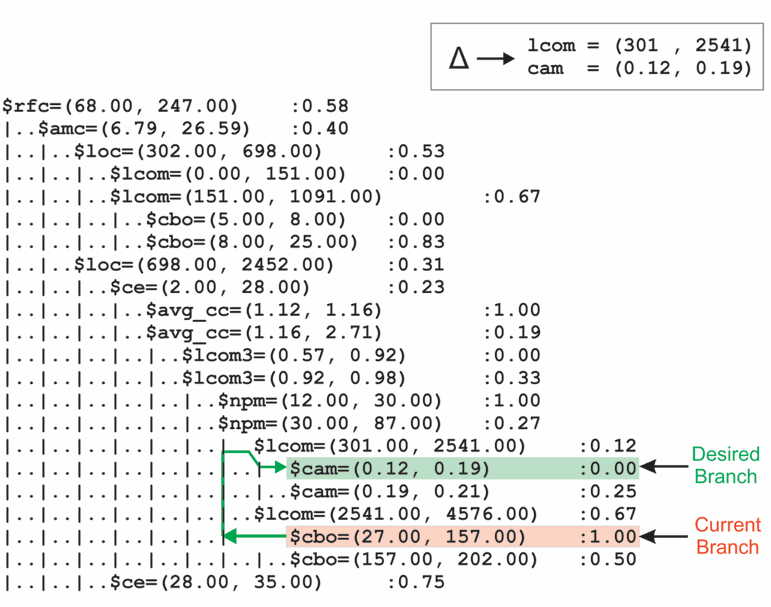
\includegraphics[width=\linewidth]{XTREE_samp.png}
\end{minipage}
~\hrule~
 \caption{A brief tutorial on XTREE.} \label{fig:xtree_samp}
\end{figure*}
	
	
	
	\subsubsection{Enri \& Lewerentz}
	Given classes described with the  code metrics of \fig{ck},
	Enri and Lewerentz~\cite{erni96} found the   mean $\mu$ and the standard deviation $\sigma$
	of each
	code metrics. Their definition of problematic outlier was any code
	metric with a measurement greater than $\mu+\sigma$.
	Shatnawi and Alves et al.~\cite{Shatnawi10,Alves2010} depreciate
	using $\mu+\sigma$ since it does not consider the fault-proneness of classes when the thresholds are computed. Also, the method lacks  empirical verification.
	
	\subsubsection{ Shatnawi}
	Shatnawi~\cite{Shatnawi10}'s preferred alternative to $\mu+\sigma$
	is to use the VARL method (Value of Acceptable Risk Level) proposed by Bender~\cite{bender99} in his epidemiology studies.  This approach uses two
	constants to compute the thresholds which, following Shatnawi's guidance, we set to
	$p_0=p_1=0.05$.
	
	VARL encodes the defect count
	for each class as 0 (no defects known in class) or 1 (defects known in class).
	Univariate binary logistic regression is applied to learn three coefficients:  
	$\alpha$ is the intercept constant;
	$\beta$ is the coefficient for maximizing log-likelihood;
	and $p_0$ 
	measures   how well this  model predicts for  defects. A univariate logistic regression was conducted comparing metrics to defect counts. Any code metric with $p>0.05$ is ignored as being a poor defect predictor. Thresholds are then learned from the surviving metrics $M_c$ using
	an equation proposed by Bender:
	$$ \mathit{bad\; smell\; if\;} M_c > VARL$$
	\begin{equation}
		VARL = p^{-1}(p_0) =  \frac{1}{\beta }\left( {\log \left( {\frac{{{p_1}}}{{1 - {p_1}}}} \right) - \alpha } \right) 
	\end{equation}
	
	
	\subsubsection{ Alves et al.}
	Alves et al.~\cite{Alves2010} propose another approach 
	to finding thresholds that  utilizes the underlying statistical distribution and scale of the metrics. 
	Metric values for each class are weighted according to the source lines of code (SLOC) of the class. All the weighted metrics are then normalized by the sum of all weights of for the system. 
	The normalized metric values are ordered in an ascending fashion (this is equivalent to computing a density function, in which the x-axis represents the weight ratio (0-100\%), and the y-axis the metric scale).
	Alves et al. then select a percentage value (they suggest 90\%) which represents the ``normal'' values for metrics. The metric threshold, then, is the metric value for which 90\% of the classes fall below. The intuition  is that the worst code has outliers beyond 90\% of the normal code measurements. Hermans et al.~\cite{hermans15} used the
	Alves et al. method in their  2015 paper on
	exploring bad smells.
	
	For consistency with Shatnawi, we explore the correlation between the code metrics and the defect counts and  reject code metrics that are poor predictors of defects (i.e.   those  with $p > 0.05$).\footnote{Okay, why focus on Shatnawi and not the others? this statement seems out of place.}
	
	\subsubsection{Discussion of Outlier Methods}\label{sect:disc}
	The advantage of the outlier-based
	approaches is that they are simple to implement, but the approaches have   two  major disadvantages. 
	First, they are {\em verbose}. A threshold can be calculated for every metric -- so, which one should the developers focus on changing? Without a means for prioritizing the  thresholds and metrics against one another, developers may have numerous or conflicting recommendations on what to improve. Second, the outlier approaches suffers from {\em conjunctive fallacy}  discussed in the introduction. That is, while	they propose thresholds for many code metrics
	individually, they make no comment on what minimal metrics need to be changed at the same time (or whether or not those changes lead to minimization or maximization of static code measures).
	
	
	\subsection{Cluster Deltas}
	
	Cluster deltas are a general method
	for learning {\em conjunctions} of changes
	that need to be applied at the same time. 
	This approach works as follows:
	\begin{itemize}
		\item Cluster the data. 
		\item Find
		neighboring clusters $C_+,C_-$ where $C_+$ has more examples of defective
		modules than $C_-$;
		\item Compute the  delta   in code metrics between the clusters using \mbox{$\Delta = C_- - C_+ = \left\{\delta|\delta\in C_-, \delta \notin C_+\right\}$}, i.e.
		{\em towards} the cluster with lower defects;
		\item The set $\Delta$ are changes needed in defective modules of $C_+$ to
		make them more like the less-defective modules of $C_-$
	\end{itemize}
	Note that $\Delta$ is a conjunction of  recommendations.
	Since it is computed
	from neighboring clusters, the examples contain similar distributions and $\Delta$ respects the naturally occurring constraints in the data. For example,
	given a bad smell pertaining to large methods,   $\Delta$   will not  suggest lowering lines of code
	without also increasing a coupling measure. 
	Cluster deltas are used in CD~\cite{me12c} and XTREE.
	
	
	
	\subsubsection{CD}\label{sec:cdcd}
	Borges and Menzies first proposed the CD centroid delta approach to
	generate {\em conjunctions} of code metrics
	that need to be changes at the same time
	in order to reduce defects~\cite{me12c}.
	CD used the WHERE clustering algorithm developed by the
	authors for a prior application~\cite{localvsglobal}.
	Each cluster was then replaced by its centroid
	and $\Delta$ was calculated directly from the difference
	between code metrics values between one centroid
	and its nearest neighbor.
	
	
	As shown below, one drawback with with CD is that it is {\em verbose}
	since
	CD   recommended changes to all code
	metrics with different values in those two centroids. 
	This makes it hard to use CD to   critique and prune away bad smells. Further, CD will be shown to be
	not as effective
	in proposing changes to reduce defects as XTREE.
	
	\subsubsection{XTREE: Overview}
	
	XTREE  is a cluster delta algorithm
	that avoids the problem of verbose $\Delta$s.
	XTREE is our {\em primary change oracle} that makes recommendations 
	of what changes should be made to code modules.
	Instead of reasoning over cluster centroids,
	XTREE utilizes a decision tree learning approach
	to find the fewest differences between clusters of examples.
	
	
	XTREE uses a multi-interval discretizer based on an iterative dichotomization scheme, first proposed by Fayyad and Irani~\cite{fi}. This method converts the values for each code metric into a small number of nominal ranges. It works as follows:
	\begin{itemize}
		\item A code metric is split into $r$ ($r=2$) ranges, each range is of
		size $n_r$ and is associated with a set of defect counts $x$ with standard deviation
		$\sigma_r$. 
		\item The best split for that range is the one that minimizes the expected value of the
		defect variance, after the split; i.e. $\sum_r\frac{n_r}{n}\sigma_x$ (where $n=\sum_r n_r$). 
		\item This discretizer then recurses on each part of the split to find other splits in a recursive fashion. As suggested by Fayyad and Irani, minimum descriptor length (MDL) is used as a termination criterion for the recursive partitioning.
	\end{itemize}
	
	When discretization finishes, each code metric $M$ has a 
	final expected value $M_v$ for the defect standard deviation 
	across all the discretized ranges of that metric.
	Iterative dichomization sorts the metrics by $M_v$
	to find the code metric that best splits the data i.e., the code metric with smallest $M_v$. 
	
	A decision tree is then constructed on the discretized metrics. The metric that generated the best split forms the root of the tree with its discrete ranges acting as the nodes. 
	
	When all the metrics are arranged this way, the process is very similar to a hierarchical clustering algorithm that groups together code modules with similar defect counts and some shared ranges of code metrics.
	For our purposes, we score each cluster found in this way according
	to the percent of classes with known defects. For example, the last line of \fig{xtree_samp} shows a tree leaf with 75\%
	defective modules.
	
	\fig{xtree_samp} offers
	a small example of how XTREE builds
	$\Delta$ by comparing branches that lead to leaf clusters
	with different defect percentages. In this example, assume a project with a table of code metrics data describing its classes in the form of \fig{ck}. After code inspections and running test cases or operational
	tests, each such class is augmented with a defect count.
	Iterative dichomization takes that table of data and, 
	generates the tree of \fig{xtree_samp}.
	
	Once the tree is built, a class with code metric data is passed into the tree and evaluated down the tree to a leaf node (see the \textcolor{orange}{{\bf orange}} line in \fig{xtree_samp}).
	XTREE then looks for a nearby leaf node with a lower defect
	count (see the \textcolor{green}{{green}} line in \fig{xtree_samp}). For that evaluated class, XTREE proposes a bad smell
	thresholds that is  the difference between 
	\textcolor{green}{{green}} and \textcolor{orange}{{\bf orange}}. 
	
	
	\subsubsection{XTREE:   Details}
	
	Using the training data construct a decision tree as suggested above.
	
%	uses  
%	iterative dichomization to
%	divide  $N$ code modules  into  clusters of
%	size $\sqrt{N}$.
	
	Next, for each test code module, 
	find $C_+$ as follows: take each test, run it down the decision tree to find a leaf in the decision tree that mostly matches the test case.  
	After that,	find $C_-$ as follows:
	\begin{itemize}
		\item Starting at the  $C_+$ leaf, ascend $lvl\in \{0,1,2...\}$ tree levels;
		\item Identify {\em sibling} leaves; i.e. leaf clusters that can be reached from level $lvl$ that are not same as {\em current $C_+$};
		\item Find the {\em better} siblings; i.e. those 50\% (or less)
		fewer defects than $C_+$. If none found, then repeat for $lvl += 1$. Also, return \texttt{nil} if the new $lvl$ is above the root. 
		\item  Set $C_-$ to the  {\em closest} better sibling where distance is measured between the mean centroids of that sibling and {\em current}
		\ei
		Now find $\Delta = C_- - C_+$  by reflecting
		on the set difference between  conditions in the decision tree branching from $C_+$ to $C_-$. To find that delta,
		for discrete attributes, delta is the value of the {\em desired}; for numerics  expressed as ranges, the delta could be any value that lies between $\left[ LOW, HIGH\right]$ in that range (random number selected from the low and high boundaries of the that range.)
		
		
		\begin{figure*}[hbtp!]
	\small
	\begin{center}
		\begin{minipage}{.46\linewidth}
			\begin{tabular}{r@{~}|l@{~}|r@{~}|l@{~}|r@{~}|r@{~}|} \cline{2-6}
			 
				
				& \multicolumn{5}{c|}{ Data set  properties}\\ 
			 
				& \multicolumn{2}{c|}{training}   & \multicolumn{3}{c|}{testing}      \\ \cline{2-6}
				data set      & versions           & cases & versions     & cases    & \% defective             \\ \hline
				jedit    & 3.2, 4.0, 4.1, 4.2 & 1257      & 4.3          & 492          & 2 \\
				ivy      & 1.1, 1.4           & 352       & 2.0          & 352          & 11 \\
				camel    & 1.0, 1.2, 1.4      & 1819      & 1.6          & 965          & 19 \\
				ant      & 1.3, 1.4, 1.5, 1.6 & 947       & 1.7          & 745          & 22 \\
				synapse  & 1.0, 1.1           & 379       & 1.2          & 256          & 34 \\
				velocity & 1.4, 1.5           & 410       & 1.6          & 229          & 34 \\
				lucene   & 2.0, 2.2           & 442       & 2.4          & 340          & 59 \\
				poi      & 1.5, 2, 2.5        & 936       & 3.0          & 442          & 64 \\
			 xerces   & 1.0, 1.2, 1.3      & 1055      & 1.4          & 588          & 74  \\ 
			 log4j    & 1.0, 1.1           & 244       & 1.2          & 205          & 92   \\
			 xalan    & 2.4, 2.5, 2.6      & 2411      & 2.7          & 909          & 99  \\\hline 
				
				
			\end{tabular}\end{minipage}~~~~~~\begin{minipage}{.4\linewidth}
			\begin{tabular}{|rrr|rrr|rr|l} \cline{1-8}
			 
				\multicolumn{8}{|c|}{  Results from learning}\\
			 
				\multicolumn{3}{|c|}{untuned} & \multicolumn{3}{c|}{tuned} & \multicolumn{2}{c|}{change}\\
				\cline{1-8}
				
				pd & pf & good? & pd & pf & good? & pd & pf\\\cline{1-8}
				\rowcolor{celadon}55 & 29 &   & 64 & 29 & y & 9 & 0&$\star$\\
				\rowcolor{celadon}	65 & 35 & y & 65 & 28 & y & 0 & -7&$\star$\\
				49 & 31 &   & 56 & 37 &   & 5 & 6\\
				\rowcolor{celadon}	49 & 13 & y & 63 & 16 & y & 14 & 3&$\star$\\
				45 & 19 &   & 47 & 15 &   & 2 & -4\\
				78 & 60 &   & 76 & 60 &   & -2 & 0\\
				56 & 25 &   & 60 & 25 & y & 4 & 0\\
				\rowcolor{celadon}	56 & 31 &   & 60 & 10 & y & 4 & -21&$\star$\\
			\rowcolor{lavenderpink}	30 & 31 &   & 40 & 29 &   & 10 & -2&$\times$\\
				\rowcolor{lavenderpink}32 & 6 &   & 30 & 6 &   & -2 & 0&$\times$\\
				\rowcolor{lavenderpink}38 & 9 &   & 47 & 9 &   & 9 & 0&$\times$\\
				\hline 
			\end{tabular}
			
		\end{minipage}
	\end{center}    
	
	\caption{Training and test {\em data set properties} for  Jureczko data ,
		sorted by \% defective examples.
		On the right-hand-side, we show the {\em results from learning}.
		Data is usable if it has a recall of 60\% or more and false alarm of 30\% or less (and note that, after tuning, there are more usable data sets than before). Results  	\colorbox{celadon}{ marked with ``$\star$''} show large improvements in performance, after tuning
		(lower {\em pf} or higher {\em pd}).
		Data in  the  \colorbox{lavenderpink}{three bottom rows}, marked with ``$\times$'', are  performing
		poorly-- that data so many defective examples  that it  is hard for
		our learners to distinguish between classes.
	}\label{fig:j}
\end{figure*}
      
		\section{Evaluation}
		The previous section proposed numerous methods for detecting bad smells that need
		to be resolved. This section offers an experiment of the following form:
		\bi
		\item Using each method as a {\em primary change oracle} to recommend how code should be changed.
		\item Apply those changes. 
		\item Run a {\em secondary verification oracle} to assess the defect-proness of the changed code.
		\item Sort the change oracles on how well they reduce defects (as judged by the verification oracle).
		\ei
		Using this experiment, we can address the research questions dicsussed in the introduction.
		
		{\bf RQ1: Effectiveness: } which of the methods defined in Section 3 is the best change oracle for identifying what and how code modules should be changed? 
		To   answer to this question, we will assume that developers
		refactor their code until the bad smell thresholds are not violated.
		This refactoring will start with some {\em initial} code
		base that is changed to a {\em new} code base. 
		For example, if the bad smell is \mbox{{\em loc $>100$}} and a 
		code module has 500 lines of code, we reason
		optimistically that we can change that code metric
		to 100.  
		Using the secondary verification oracle,  we then predict the
		number of defects in $d_+,d_-$ in {\em initial} and {\em new}. We evaluate the performance of XTREE, CD, Shatnawi, and Alves methods in setting bad smell thresholds.
		The best bad smell threshold method is the one that maximizes
		\begin{equation}\label{eq:diff}
			\mathit{improvement} = 100* \left(1 - \frac{ d_- }{ d_+}\right)
		\end{equation}
		
		
		{\bf RQ2: Succinctness: } which of the Section 3 methods recommended changes to the fewest code attributes?
		To answer this question, we will report the frequency at which different attributes are selected in repeated runs of our oracles.
		
		{\bf RQ3: Stopping: }    How effective is XTREE at offering   ``stopping points'' (i.e. clear guidance on what {\em not} to do)?   
		To answer this point, we will report how often XTREE's recommendations {\em omit} a code attribute. 
		Note that the {\em more often} XTREE omits an attribute, the more likely it is {\em not} to endorse a bad smell based on the omitted
		attribites.
		
		{\bf RQ4: Stability:} Across different projects, how variable are the changes recommended by XTREE?   To answer this
		question, we conduct a large scale ``what if'' study that reports all the possible recommendations XTREE might make.
		We then count how often attributes are {\em not} found in the recommendations arising from this ``what if'' study.
		
		{\bf RQ5: Conjunctive Fallacy:} Is  it  always  useful  to  apply \eq{df}; i.e.   make  code  better  by  reducing  the  values  of multiple code attributes? To answer this question, we will look at the {\em direction of change} seen in the {\bf RQ4} study; i.e.
		how often does XTREE recommend decreasing or increasing a static code attribute.
		
		
		
		
		
		\subsection{Test Data}\label{sect:tesd}
		
		To explore these research questions,
		we used data from
		Jureczko et al.'s collection of object-oriented Java systems~\cite{jureczko10}. To access that data, go to   git.io/vGYxc.
		The Jureczko data records the number of known defects for each class using a post-release bug tracking system. The classes are described in terms of nearly two dozen metrics included in the Chidamber and Kemerer metric suite, such as number of children (noc), lines of code (loc), etc. For details on the Jureczko code
		metrics, see  \fig{ck}. For details on the rows and versions
		of that data, see the left-hand-side columns of \fig{jur}.
		
		
		
		
		\subsection{Secondary verification Oracles}
		\label{sect:eval}
		
		As mentioned in the introduction, our proposed framework has two oracles:
		a primary change oracle (XTREE) and the secondary verification oracle described in this section.
		
		It can be difficult  to judge the  effects of removing bad smells.
		Refactored code cannot be assessed just by a rerun of the the test
		suite (since refactorings are supposed to preserve behavior). 
		% waiting to observe 
		% code refactorings is meant to
		% preserve the behavior of the system (i.e. the same tests
		% should pass before and after the refactoring). 
		Also, it many not be practical
		to assessing refactorings by making the
		refactorings,  then seeing what happens to that code for the rest
		of the project. In a test-driven agile project, as
		SCRUM meetings change what stories are implemented next,
		the operational profile that lead to defects in the old
		code may not be repeated in future executions. 
		
		To resolve this  problem, SE researchers such as 
		Cheng et al.~\cite{Cheng10}, O'Keefe et al.~\cite{OKeeffe08,OKeeffe07},
		Moghadam~\cite{Moghadam2011} and Mkaouer et al.~\cite{Mkaouer14}
		use a {\em secondary verification oracle} (which is learned separately
		to the primary oracle) that   assesses
		how defective is the code before and after some
		refactoring. 
		For their second oracle,
		Cheng, O'Keefe, Moghadam and  Mkaouer et al. use the QMOOD hierarchical
		quality model~\cite{Bansiya02}.
		A shortcoming of QMOOD
		is that quality models learned from other projects
		may perform poorly when applied to new projects~\cite{localvsglobal}.
		Hence, for this study, we  eschew
		older quality models like QMOOD. Instead, we use
		Random Forests~\cite{Breiman2001} to learn defect predictors
		from OO code metrics.
		Note that, unlilke QMOOD, such measurements 
		are specific to the project, and the measurements can be reconstructed and the predictors rebuilt for other projects.
		
		Random Forests are a decision tree learning method but
		instead of building one tree, hundreds are built using
		randomly selected subsets of the data. The final predictions
		come from averaging the predictions over all the trees.
		Recent studies endorsed the use
		of  Random Forests for  defect prediction~\cite{lessmann}.
		
		\fig{j} shows   studies with Random Forests and
		the Jureczko data. Given   $V$ released versions, we test on version $V$ and train on the available data from $V-1$ earlier releases (as shown in \fig{j}. Note the   \colorbox{lavenderpink}{three bottom rows}   marked with $\times$: these contain predominately defective classes (two-thirds, or more).  In such data, it is hard to distinguish good examples (due to all the bad examples). 
		
		In order to identify the presence (or absence) of defects, we can   use Boolean classes in the  Jureczko data ( \texttt{True} if defects \textgreater 0; \texttt{False} if defects = 0). For such data, the quality of the predictor can be measured using (a) the  probability of detection (a.k.a. ``pd'' or recall):  the percent of faulty classes in the test data detected by the {\em predictor}; and (b) the  probability of false alarm (a.k.a. ``pf''): the percent of non-fault classes that are {\em predicted} to be defective.
		
		The ``untuned'' columns of \fig{j}
		show a preliminary study. This study used
		Random Forest with its ``off-the-shelf'' tunings (i.e.  
		100 trees per forest).  
		The forests were built from training data and applied to test data
		not seen during training.  In this
		study, we called a data set ``usable'' if   Random Forest was able to classify the instances with a performance threshold of $\mathit{pd}\ge 60 \wedge \mathit{pf} \le 30$\% (determined from standard results in other publications~\cite{me07b}). Note that no  data set meet
		that criteria.
		
		The ``tuned'' columns of \fig{j} show that we can salvage some of the data sets. We applied both the SMOTE algorithm and differential evolution to improve the performance of the classifier. Pelayo and Dick~\cite{pelayo07} report that defect prediction is improved by SMOTE~\cite{Chawla2002}; i.e. an over-sampling of minority-class examples and an under-sampling of majority-class examples. Fu et al.~\cite{fu:ase15} report that parameter tuning with differential evolution~\cite{storn97} can quickly explore the tuning options of Random Forest to find better settings for the (e.g.) size of the forest, the termination criteria
		for tree generation, etc. We note that SMOTE-ing and
		parameter tunings were applied to the training data only and not to the test data.
		
		The rows \colorbox{celadon}{marked with a $\star$} in \fig{j} show data sets whose performance was improved remarkably by these techniques. For example, in {\em poi}, the recall increased by 4\% while the false alarm rate dropped by 21\%. However, as might have been expected, we could not salvage the data sets in the  three bottom rows.
		
		We eliminate the data sets for which we could not build an adequately performing Random Forest classifier with $\mathit{pd}\ge 60 \wedge \mathit{pf} \le 30$\%. Thus, our analysis uses the {\em jedit, ivy, ant, lucene} and {\em poi} for evaluating recommended changes.
		
		
		
%		\subsection{Experiment}
%		Describe what you actually did, including: 
%		\bi
%		\item what metrics you used to identify refactorings using the 4 methods. Also, what is your data here? Is it the rows and columns of CK/OO metrics for each file?
%		\item how you applied the recommended changes from the 4 methods to the data 
%		\item how you chose to handle the ``conjuctive fallacy' of non-CD, non-XTREE methods
%		\item What are you considering correct, i.e., if the change to the code metrics yielded a non-defective (i.e., \# defects = 0) file, then the refactoring is good. 
%		\item how you aggregated the results from your 40 runs for each method
%		\ei
%		
		
		\subsection{Statistics}
		
		
		We use 40 repeated runs, each with different random number seeds (we use 40 since that is  more than the 30 samples  needed to satisfy the central limit theorem). Each run collects the \eq{diff} values.
		We use multiple runs since two of our methods use some random choices: CD uses the  stochastic WHERE clustering algorithm~\cite{localvsglobal}
		while XTREE non-deterministically picks thresholds randomly from
		the high and low boundary of a range. 
		Hence, to compare all
		four methods, we must run the analysis many times. 
		
		
		
		\begin{figure}[!htbp]
%{\scriptsize \textbf{Ant}\\[0.1cm]}


{\scriptsize \hspace{3.5cm}\underline{Observed Improvements (from \eq{diff})}}\vspace{2mm}
 

{\scriptsize \textbf{Ant}~~~~~~~~ \begin{tabular}{{l@{~~~~}l@{~~~~}|r@{~~~~}r@{}c@{~~~}r}}
\arrayrulecolor{lightgray}
\rowcolor{lightgray}\textbf{Rank} & \textbf{Treatment} & \textbf{Median} & \textbf{IQR~~~} & \\
  1 &         XTREE &    56   &  21  & \quart{54}{25}{65}{1} \\
\hline  2 &        Alves &    32   &  17  & \quart{28}{20}{37}{1} \\
\hline  3 &     Shatnawi &    15   &  4.2 & \quart{15}{6}{18}{1} \\
  3 &           CD &    12   &  0  & \quart{15}{0}{15}{6} \\
\hline \end{tabular}}\\

%{\scriptsize \textbf{Lucene}\\[0.1cm]}
%{\scriptsize \textbf{Poi}\\[0.1cm]}
{\scriptsize 

\textbf{Poi}~~~~~~~~ \begin{tabular}{{l@{~~~~}l@{~~~~}|r@{~~~~}r@{~~}c@{}r}}
\arrayrulecolor{lightgray}
\rowcolor{lightgray}\textbf{Rank} & \textbf{Treatment} & \textbf{Median} & \textbf{IQR~~~} & \\
        1 &         XTREE &    20   &  16  & \quart{39}{40}{51}{2} \\
\hline  2 &        Alves &    14   &  16  & \quart{21}{41}{37}{2} \\
\hline  3 &           CD &    11   &  0  & \quart{23}{0}{23}{7} \\
        3 &     Shatnawi &    8   &  1  & \quart{19}{5}{21}{2} \\
\hline \end{tabular}}\\

{\scriptsize \textbf{Lucene}~ \begin{tabular}{{l@{~~~~}l@{~~~~}|r@{~~~~}r@{~~}c@{}r}}
\arrayrulecolor{lightgray}
\rowcolor{lightgray}\textbf{Rank} & \textbf{Treatment} & \textbf{Median} & \textbf{IQR~~~} & \\
        1 &         XTREE &    16   &  6  & \quart{50}{29}{71}{4} \\
        1 &     Shatnawi  &    15   &  2  & \quart{63}{10}{67}{4} \\
\hline  2 &           CD  &    13   &  0  & \quart{55}{0}{55}{6} \\
\hline  3 &        Alves  &    9   &  4  & \quart{33}{19}{42}{4} \\
\hline \end{tabular}}\\


%{\scriptsize \textbf{Ivy}\\[0.1cm]}
{\scriptsize \textbf{Ivy}~~~~~~~~ \begin{tabular}{{l@{~~~~}l@{~~~~}|r@{~~~~}r@{~~}c@{}r}}
\arrayrulecolor{lightgray}
\rowcolor{lightgray}\textbf{Rank} & \textbf{Treatment} & \textbf{Median} & \textbf{IQR~~~} & \\
        1 &        Alves &    67   &  20  & \quart{58}{21}{71}{1} \\
\hline  2 &         XTREE &    52   &  22  & \quart{42}{24}{55}{1} \\
\hline  3 &           CD &    35   &  0  & \quart{27}{0}{27}{2} \\
\hline  4 &     Shatnawi &    20   &  7  & \quart{18}{8}{21}{1} \\
\hline \end{tabular}}\\

%{\scriptsize \textbf{Jedit}\\[0.1cm]}

{\scriptsize  \textbf{Jedit}~~~~~ \begin{tabular}{{l@{~~~}l@{~~~~}|r@{~~~~}r@{~~}c@{}r}}
\arrayrulecolor{lightgray}
\rowcolor{lightgray}\textbf{Rank} & \textbf{Treatment} & \textbf{Median} & \textbf{IQR~~~} & \\
  1 &        Alves &    36   &  7  & \quart{60}{10}{66}{1} \\
  1 &        XTREE &    36   &  0  & \quart{66}{0}{66}{2} \\
  1 &     Shatnawi &    36   &  9  & \quart{53}{13}{66}{1} \\
  1 &          CD &    36   &  0  & \quart{66}{0}{66}{2} \\
\hline \end{tabular}}\\
\caption{Results for {\bf RQ1} from the
Jureczko   data sets.  Results from 40 repeats.
Values come from \eq{diff}.
Values near 0
imply no improvement,
{\em Larger} median values are {\em better}. 
Note that XTREE and Alves are usually best and CD and Shatnami
are usually worse.}
\label{fig:jur}
\end{figure}

% ## ant

% {\scriptsize \begin{tabular}{l@{~~~}l@{~~~}r@{~~~}r@{~~~}c}
% \arrayrulecolor{lightgray}
% \textbf{XTREE} & \textbf{Treatment} & \textbf{Median} & \textbf{IQR} & \\\hline
%   1 &     Shatnawi &    15.66  &  4.82 & \quart{15}{6}{18}{1} \\
% \hline  2 &        Alves &    32.53  &  17.47 & \quart{28}{20}{37}{1} \\
% \hline  3 &         XTREE &    56.02  &  21.68 & \quart{54}{25}{65}{1} \\
% \hline \end{tabular}}


% ## ivy

% {\scriptsize \begin{tabular}{l@{~~~}l@{~~~}r@{~~~}r@{~~~}c}
% \arrayrulecolor{lightgray}
% \textbf{XTREE} & \textbf{Treatment} & \textbf{Median} & \textbf{IQR} & \\\hline
%   1 &     Shatnawi &    20.0  &  7.5 & \quart{18}{8}{21}{1} \\
% \hline  2 &         XTREE &    52.5  &  22.5 & \quart{42}{24}{55}{1} \\
% \hline  3 &        Alves &    67.5  &  20.0 & \quart{58}{21}{71}{1} \\
% \hline \end{tabular}}


% ## jedit

% {\scriptsize \begin{tabular}{l@{~~~}l@{~~~}r@{~~~}r@{~~~}c}
% \arrayrulecolor{lightgray}
% \textbf{XTREE} & \textbf{Treatment} & \textbf{Median} & \textbf{IQR} & \\\hline
%   1 &     Shatnawi &    36.36  &  9.09 & \quart{53}{13}{53}{1} \\
%   1 &         XTREE &    36.36  &  0.0 & \quart{53}{0}{53}{1} \\
%   1 &        Alves &    45.45  &  27.28 & \quart{39}{40}{66}{1} \\
% \hline \end{tabular}}


% ## lucene

% {\scriptsize \begin{tabular}{l@{~~~}l@{~~~}r@{~~~}r@{~~~}c}
% \arrayrulecolor{lightgray}
% \textbf{XTREE} & \textbf{Treatment} & \textbf{Median} & \textbf{IQR} & \\\hline
%   1 &        Alves &    9.85  &  4.44 & \quart{33}{19}{42}{4} \\
% \hline  2 &     Shatnawi &    15.76  &  2.45 & \quart{63}{10}{67}{4} \\
%   2 &         XTREE &    16.75  &  6.9 & \quart{50}{29}{71}{4} \\
% \hline \end{tabular}}


% ## poi

% {\scriptsize \begin{tabular}{l@{~~~}l@{~~~}r@{~~~}r@{~~~}c}
% \arrayrulecolor{lightgray}
% \textbf{XTREE} & \textbf{Treatment} & \textbf{Median} & \textbf{IQR} & \\\hline
%   1 &     Shatnawi &    8.53  &  1.78 & \quart{19}{5}{21}{2} \\
% \hline  2 &        Alves &    14.95  &  16.38 & \quart{21}{41}{37}{2} \\
% \hline  3 &         XTREE &    20.64  &  16.02 & \quart{39}{40}{51}{2} \\
% \hline \end{tabular}}


		
		To rank these 40 numbers collected from CD, XTREE, Shatnawi, and Alves et al., we use the Scott-Knott test recommended by Mittas and Angelis~\cite{mittas13}. 
		Scott-Knott is a top-down clustering approach used to rank different
		treatments. If that clustering finds an interesting division of the data, then
		some statistical test is applied to the two divisions to check if they
		are statistically significant different. If so, Scott-Knott recurses
		into both halves.
		
		To  apply Scott-Knott,
		we
		sorted a list of  $l=40$ values of \eq{diff} values found in  $ls=4$ different methods. 
		Then, we split $l$ into sub-lists $m,n$ in order to maximize the expected value of differences in the observed performances before and after divisions. E.g. for lists $l,m,n$ of size $ls,ms,ns$ where $l=m\cup n$: \[E(\Delta)=\frac{ms}{ls}abs(m.\mu - l.\mu)^2 + \frac{ns}{ls}abs(n.\mu - l.\mu)^2\]
		We then apply a apply a statistical hypothesis test $H$ to check
		if $m,n$ are significantly different  (in our case, the conjunction of A12 and bootstrapping). If so, Scott-Knott recurses on the splits. In other words, we divide the data if \textit{both} bootstrap sampling and effect size test agree that a division is statistically significant (with a confidence of 99\%) and not a small effect ($A12 \ge 0.6$).
		For a justification of the use of non-parametric bootstrapping, see Efron \& Tibshirani~\cite[p220-223]{efron93}. For a justification of the use of effect size tests see Shepperd\&MacDonell~\cite{shepperd12a}; Kampenes~\cite{kampenes07}; and Kocaguenli et al.~\cite{Kocaguneli2013:ep}. These researchers warn that even if a hypothesis test declares two populations to be ``significantly'' different, then that result is misleading if the ``effect size'' is very small. Hence, to assess the performance differences we first must rule out small effects using A12, a test   recently endorsed by Arcuri and Briand at ICSE'11~\cite{arcuri11}.
		
		The Scott-Knott  results are presented in the form of line diagrams like those shown on the right-hand-side of \fig{jur}.
		The black dot shows the median \eq{diff} values and the horizontal lines stretch 
		from the 25th percentile to the 75th percentile (the inter-quartile range, IQR).
		As an example of how to read this table, consider the {\em Ant}
		results. Those rows are  sorted on the median values of each method. Note that all the methods have \eq{diff} \textgreater $ 0\%$; i.e. all these methods reduced the expected value of the performance score in that experiment while XTREE achieved the greatest reduction (of 56\% from the original value).
		These results table has a  left-hand-side  {\bf Rank} column, computed using the
		Scott-Knott test described above. In the {\em Ant}
		results, XTREE is ranked the best, while CD is  ranked   worst.
		
		% Please add the following required packages to your document preamble:
% \usepackage{multirow}
% \usepackage[table,xcdraw]{xcolor}
% If you use beamer only pass "xcolor=table" option, i.e. \documentclass[xcolor=table]{beamer}
\newcommand{\ZZ}{.}
\begin{figure*}
\renewcommand{\baselinestretch}{0.8} 
\scriptsize  
\centering

\label{my-label}
                  
\begin{tabular}{c|rrrr|rrrr|rrrr|rrrr|rrrr}
\multicolumn{1}{c}{\cellcolor[HTML]{EFEFEF}{\color[HTML]{000000} }} & \multicolumn{4}{c}{\cellcolor[HTML]{EFEFEF}{\color[HTML]{000000} Ant}} & \multicolumn{4}{c}{\cellcolor[HTML]{EFEFEF}{\color[HTML]{000000} Ivy}} & \multicolumn{4}{c}{\cellcolor[HTML]{EFEFEF}{\color[HTML]{000000} Lucene}} & \multicolumn{4}{c}{\cellcolor[HTML]{EFEFEF}{\color[HTML]{000000} Jedit}} & \multicolumn{4}{c}{\cellcolor[HTML]{EFEFEF}{\color[HTML]{000000} Poi}} \\
\multicolumn{1}{c@{}}{\multirow{-2}{*}{\cellcolor[HTML]{EFEFEF}{\color[HTML]{000000} Features}}} & \multicolumn{1}{c@{}}{\cellcolor[HTML]{EFEFEF}{\color[HTML]{000000} XTREE}} & \multicolumn{1}{c@{}}{\cellcolor[HTML]{EFEFEF}{\color[HTML]{000000} CD}} & \multicolumn{1}{c@{}}{\cellcolor[HTML]{EFEFEF}{\color[HTML]{000000} Alves}} & \multicolumn{1}{c@{}}{\cellcolor[HTML]{EFEFEF}{\color[HTML]{000000} Shatn}} & \multicolumn{1}{c@{}}{\cellcolor[HTML]{EFEFEF}{\color[HTML]{000000} XTREE}} & \multicolumn{1}{c@{}}{\cellcolor[HTML]{EFEFEF}{\color[HTML]{000000} CD}} & \multicolumn{1}{c@{}}{\cellcolor[HTML]{EFEFEF}{\color[HTML]{000000} Alves}} & \multicolumn{1}{c@{}}{\cellcolor[HTML]{EFEFEF}{\color[HTML]{000000} Shatn}} & \multicolumn{1}{c@{}}{\cellcolor[HTML]{EFEFEF}{\color[HTML]{000000} XTREE}} & \multicolumn{1}{c@{}}{\cellcolor[HTML]{EFEFEF}{\color[HTML]{000000} CD}} & \multicolumn{1}{c@{}}{\cellcolor[HTML]{EFEFEF}{\color[HTML]{000000} Alves}} & \multicolumn{1}{c@{}}{\cellcolor[HTML]{EFEFEF}{\color[HTML]{000000} Shatn}} & \multicolumn{1}{c@{}}{\cellcolor[HTML]{EFEFEF}{\color[HTML]{000000} XTREE}} & \multicolumn{1}{c@{}}{\cellcolor[HTML]{EFEFEF}{\color[HTML]{000000} CD}} & \multicolumn{1}{c@{}}{\cellcolor[HTML]{EFEFEF}{\color[HTML]{000000} Alves}} & \multicolumn{1}{c@{}}{\cellcolor[HTML]{EFEFEF}{\color[HTML]{000000} Shatn}} & \multicolumn{1}{c@{}}{\cellcolor[HTML]{EFEFEF}{\color[HTML]{000000} XTREE}} & \multicolumn{1}{c@{}}{\cellcolor[HTML]{EFEFEF}{\color[HTML]{000000} CD}} & \multicolumn{1}{c@{}}{\cellcolor[HTML]{EFEFEF}{\color[HTML]{000000} Alves}} & \multicolumn{1}{c@{}}{\cellcolor[HTML]{EFEFEF}{\color[HTML]{000000} Shatn}} \\
wmc & \ZZ & 92 & 100 & 100 & 18 & 95 & 100 & 100 & 89 & 95 & 100 & \ZZ &\ZZ& 63 & \ZZ &\ZZ& \ZZ & 100 & 100 &\ZZ\\
dit & \ZZ & 77 & 100 & \ZZ & \ZZ & 87 & 100 & \ZZ & \ZZ & 80 & 100 & \ZZ &\ZZ& 72 & 100 & 100 & \ZZ & 46 & 100 &\ZZ\\
noc & \ZZ & 20 & 100 & \ZZ & \ZZ & \ZZ & 100 & \ZZ & \ZZ & 26 & \ZZ &\ZZ& \ZZ &\ZZ& \ZZ &\ZZ& \ZZ &\ZZ& \ZZ &\ZZ\\
cbo & 88 & 99 & 100 & 100 & 91 & 100 & 100 & 100 & 60 & 94 & 100 & 100 & \ZZ & 100 & 100 & \ZZ & 1 & 74 & 100 &\ZZ\\
rfc & 100 & 100 & 100 & \ZZ & 8 & 95 & 100 & \ZZ & 10 & 83 & 100 & \ZZ & 100 & 100 & 100 & 100 & 100 & 95 & 100 &\ZZ\\
lcom & \ZZ & 98 & 100 & 100 & 15 & 100 & 100 & 100 & \ZZ & 94 & 100 & \ZZ &\ZZ& 100 & 100 & \ZZ &\ZZ& 100 & 100 & 100 \\
ca & \ZZ & 93 & 100 & \ZZ & 7 & 95 & 100 & \ZZ & 40 & 89 & 100 & \ZZ &\ZZ& 63 & 100 & 100 & \ZZ & 74 & 100 &\ZZ\\
ce & 5 & 100 & 100 & \ZZ & \ZZ & 97 & 100 & \ZZ &\ZZ& 90 & 100 & \ZZ &\ZZ& 100 & 100 & 100 & \ZZ & 64 & 100 &\ZZ\\
npm & \ZZ & 88 & 100 & \ZZ & 8 & 97 & 100 & \ZZ &\ZZ& 93 & 100 & 100 & \ZZ & 100 & 100 & \ZZ &\ZZ& 100 & 100 &\ZZ\\
lcom3 & \ZZ & 90 & 100 & \ZZ & 7 & 95 & 100 & \ZZ & 13 & 79 & 100 & 100 & \ZZ & 63 & 100 & 100 & \ZZ & 92 & 100 & 100 \\
loc & 100 & 99 & 100 & 100 & 97 & 97 & 100 & 100 & 60 & 100 & 100 & 100 & \ZZ & 100 & \ZZ & 100 & 100 & 100 & 100 & 100 \\
dam & \ZZ & 21 & 100 & \ZZ & \ZZ & 22 & 100 & \ZZ &\ZZ& 55 & 100 & \ZZ &\ZZ& 45 & 100 & 100 & \ZZ & 73 & 100 &\ZZ\\
moa & \ZZ & 67 & 100 & \ZZ & \ZZ & 82 & 100 & \ZZ &\ZZ& 60 & 100 & 100 & \ZZ & 54 & 100 & 100 & \ZZ & 58 & 100 &\ZZ\\
mfa & 5 & 93 & 100 & \ZZ & \ZZ & 90 & 100 & \ZZ & 5 & 80 & 100 & \ZZ &\ZZ& 72 & 100 & \ZZ &\ZZ& 72 & 100 &\ZZ\\
cam & \ZZ & 99 & 100 & 100 & 84 & 100 & 100 & 100 & 10 & 94 & 100 & \ZZ &\ZZ& 100 & 100 & \ZZ &\ZZ& 98 & 100 & 100 \\
ic & \ZZ & 52 & 100 & 100 & \ZZ & 70 & \ZZ &\ZZ& \ZZ & 68 & 100 & \ZZ &\ZZ& 36 & 100 & \ZZ &\ZZ& 43 & 100 & 100 \\
cbm & \ZZ & 59 & 100 & \ZZ & \ZZ & 85 & \ZZ &\ZZ& \ZZ & 71 & 100 & \ZZ &\ZZ& 36 & 100 & 100 & \ZZ & 67 & 100 &\ZZ\\
amc & \ZZ & 99 & \ZZ & \ZZ & \ZZ & 95 & 100 & \ZZ & 30 & 100 & \ZZ & \ZZ & \ZZ & 100 & 100 & 100 & \ZZ & 97 & \ZZ &\ZZ\\
max cc & \ZZ & 87 & 100 & 100 & \ZZ & 85 & 100 & 100 & \ZZ & 71 & \ZZ &\ZZ& \ZZ & 45 & 100 & \ZZ &\ZZ& 63 & 100 &\ZZ\\
avg cc & 12 & 99 & 100 & 100 & \ZZ & 95 & 100 & 100 & 13 & 98 & \ZZ &\ZZ& \ZZ & 100 & 100 & 100 & \ZZ & 92 & 100 & \ZZ\\\hline
\end{tabular}
\caption{Results for {\bf RQ2}.
Percentage counts of  how often an approach recommends changing a code metric
(in 40 runs). ``100'' means that this code metric
was always recommended. Cells marked with ``.'' indicate  0\%. For the Shatnami and Alves et al.
columns,  metrics score 0\% if they always fail the $p \le 0.05$ test of \tion{shatnawi}.
For CD, cells are blank when two centroids have the same value for the same code
metrics. For XTREE, cells are blanks when they do not appear in the delta
between branches.  Note
that XTREE mentions specific code metrics
far fewer times than other methods.}\label{fig:counts}
\end{figure*}
		\section{Results}
		
		
		\begin{figure*}[!t]
			\centering
			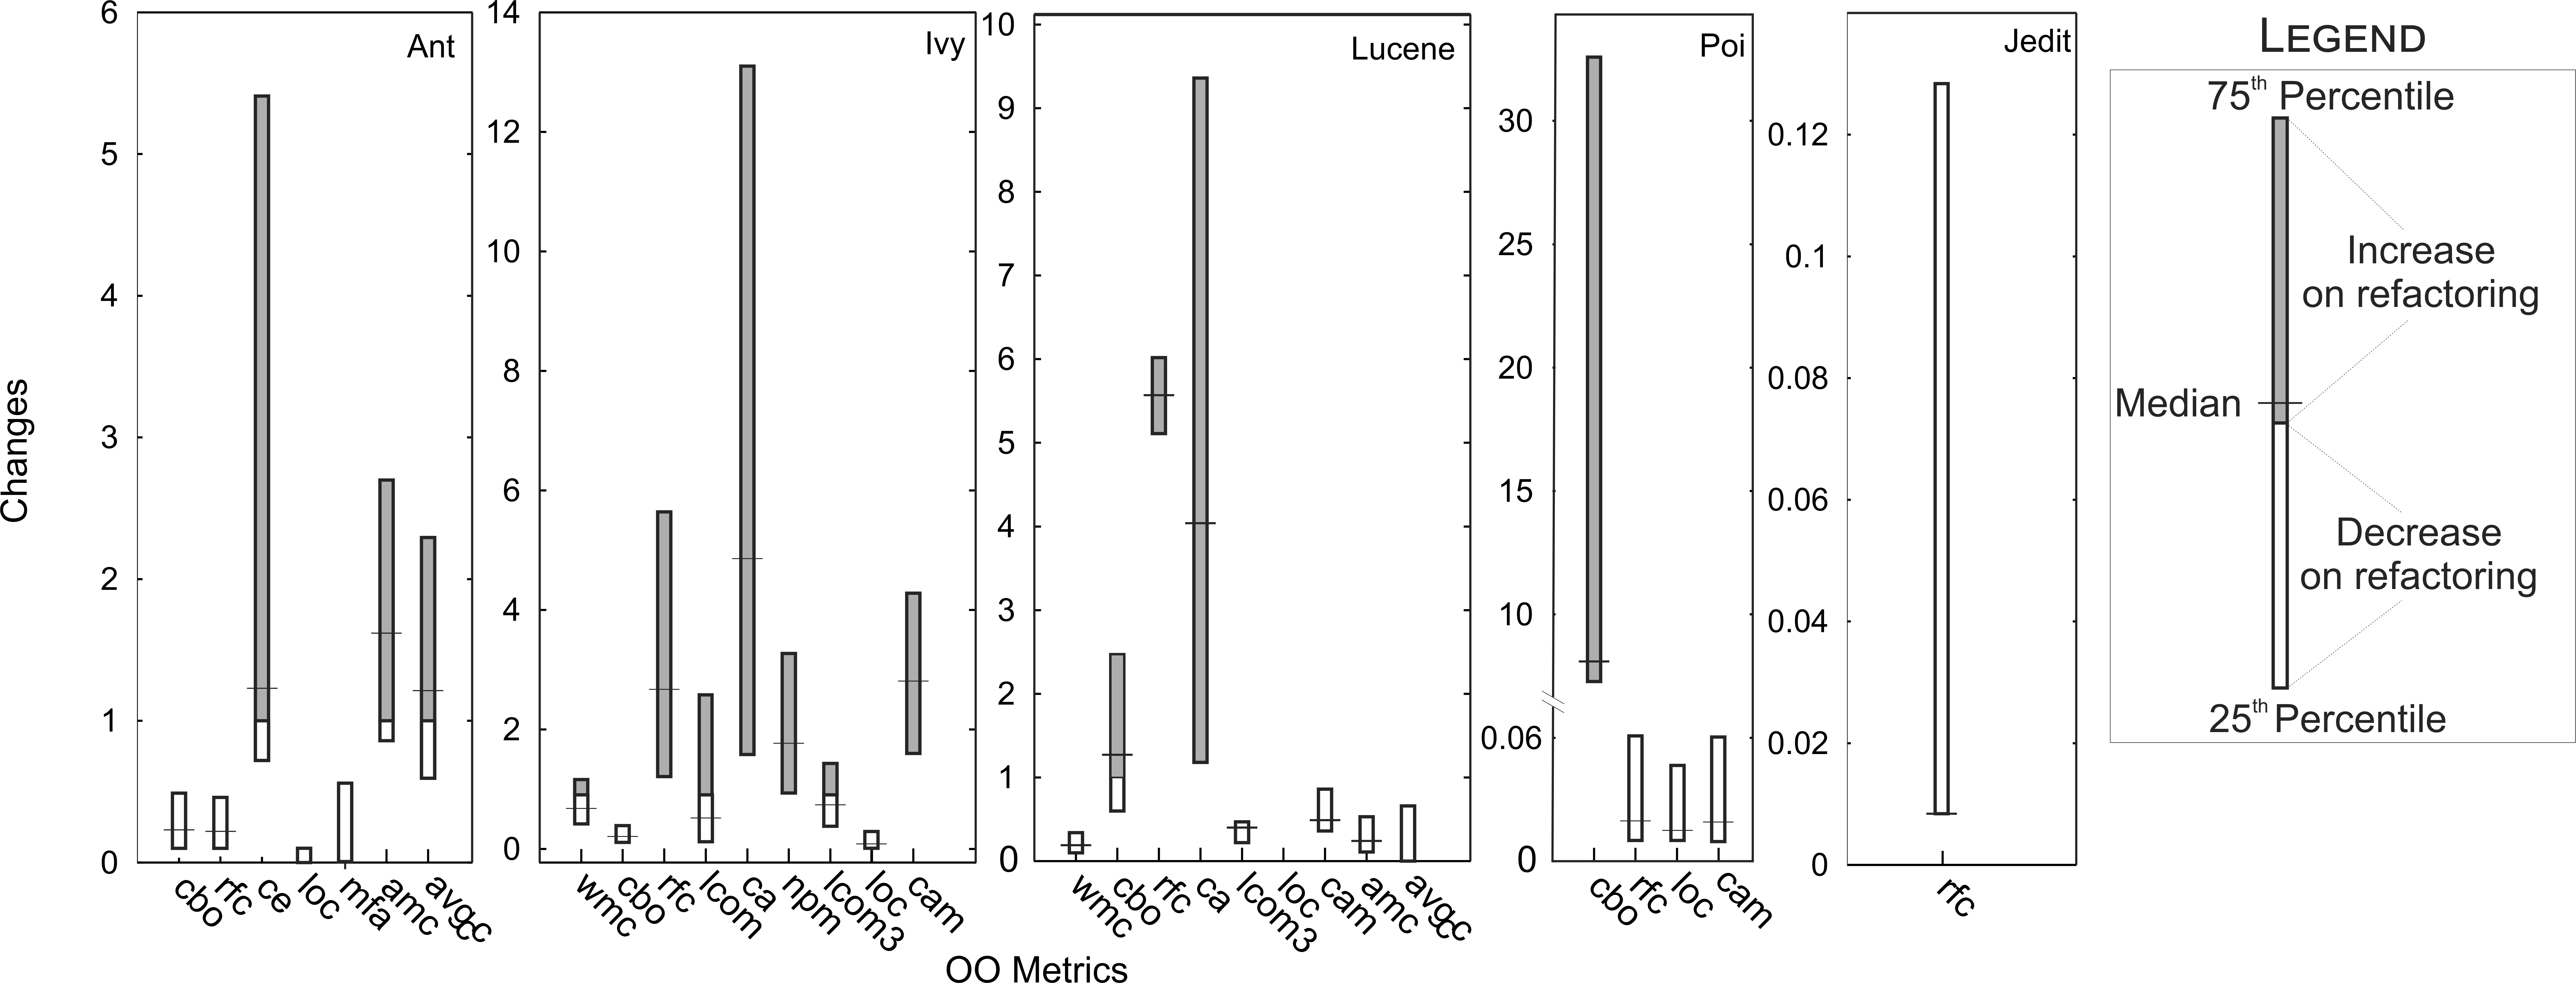
\includegraphics[width=\linewidth]{figs/changes01.png}
			\caption{Results  from XTREE.
				While \fig{counts} are the {\em number} of times a code metric was changed,
				this  figure shows {\em how far} each code metric was changed. Each vertical bar
				marks the 27,50,75th percentile change seen in 40 repeats.
				All numbers are ratios of initial to final values.
				All bar regions marked in gray show {\em increases}.
				The interesting feature of these results are that many
				of the changes proposed by XTREE require {\em increases}
				(this puzzling observation is explained in the text).}
			\label{fig:changes}
		\end{figure*}
		
		
		
		\subsection{RQ1: Effectiveness}
		
		{\em Which of the methods defined in Section 3 is the best change oracle for identifying what and howcode modules should be changed? }
		
		\fig{jur} shows the comparison results.  The Alves and Shatnawi
		entries show the net effects of applying \eq{df} where the $t_i$ values were found by Alves and Shatnawi.
		In this part of the  analysis,
		we applied Scott-Knott to all the \eq{diff} values
		seen when code metrics were changed
		according to the  Alves and Shatnawi
		
		
		Two data sets are very responsive to defect reduction suggestions:
		Ant, and Ivy (both of which show best case improvements over 50\%).
		The  expected value of defects  
		is changed less in Jedit. This data sets' results
		surprisingly uniform; i.e.   all methods
		find the same ways to reduce the expected number of
		defects.   For an explanation of the Jedit uniformity, see \tion{inc}.
		
		Two data sets are not very responsive to defect reduction:
		Poi and Lucene. The reason for this can be see in \fig{j}:
		both these data sets contain more than 50\% defective modules.
		In that space, all our  methods lack a large sample of
		defect-free examples. 
		
		Also consider the relative
		rank of the different approaches,
		CD and Shatnawi usually  perform comparatively worse while  XTREE gets top ranked position the most
		number of times. That said, Alves sometimes beats XTREE (see Ivy)
		while sometimes it ties (see Jedit).
		
		In summary, our {\bf Result1} is  that, of the change orcales studies here,
		XTREE is the best oracle on how to change code modules (in order to reduce defects).
		
		% Please add the following required packages to your document preamble:
% \usepackage{graphicx}
\begin{figure*}
\centering
\resizebox{\textwidth}{!}{%
\begin{tabular}{l|c|c|c|c|c|c|c|c|c|c|c|c|c|c|c|c|c|c|c|c}
         & wmc & dit & noc & cbo & rfc & lcom & ca & ce & npm & lcom3 & loc & dam & moa & mfa & cam & ic & cbm & amc & max\_cc & avg\_cc \bigstrut\\ \hline
Ant      &  & & & $-$ &$-$&  & &$+$& & &$-$& & &$-$& & &  &$+$&     &$+$\bigstrut\\ \hline

Ivy      &$-$& & &$-$&$+$&$-$&$+$& &$-$&$-$&$-$& & & &$+$& & & &     &      \bigstrut\\ \hline

Poi      & & & &$+$&$-$& & & & & &$-$& & & &$-$& & & & & \bigstrut\\ \hline

Lucene   &$-$& & &$+$&$+$& &$+$& & &$-$&$-$& & & &$-$& & &$-$& &$-$\bigstrut\\ \hline

Jedit    & & & & &$-$& & & & & & & & & & & & & & &     \bigstrut\\ 

\end{tabular}}

\caption{Direct of changes seen in  
a comparison of statistically significantly different static code attributes measures seen in the clusters found by XTREE. Each dataset contains 20 Static Code Metrics (for a description of each of these metrics, please refer to~\cite{me12d}). The rows contain the datasets, and the columns denote the metrics. A ``$+$'' symbol represents a recommendation that requires a significant statistical increase (with a p-value$\le$0.05), and likewise, a ``$-$'' represents a significant statistical decrease.} 
\label{fig:multcomp}
\end{figure*}
		
		\subsection{RQ2: Verbosity}
		
		{\em Which of the Section 3 methods recommended changes to the fewest code attributes?}
		
		\fig{counts} shows the frequency with which the methods
		recommend changes to specific code metrics.
		Note that XTREE proposes thresholds to
		few code metrics compared to the other approaches. 
		
		% COMMENT From LL: This is such a strange way of putting this lesson, and you haven't actually evaluated this.
		% 
		
		Hence, our {\bf Result2} is that, of all the code change oracles studied here, XTREE recommended far fewest changes to static code measures.
		Note only that,   combining  \fig{jur} with \fig{counts}, we   see that
		even though XTREE proposes changes to far fewer code metrics, those few
		code metrics are usually just as effective (or
		more effective) than the multiple
		thresholds
		proposed by CD, Shatnawi or Alves.  That is, XTREE proposes
		{\em fewer} and better thresholds than the other approaches studied here.
		
		
		
		\subsection{RQ3: Stopping}
		
		{\em  How effective is XTREE at offering   ``stopping points'' (i.e. clear guidance on what not to do)?}
		
		The {\bf RQ2} results showed that XTREE's recommendations are small in a {\em relative sense}; i.e. they are 
		relatively smaller than the other methods studied here.
		Note only that, but XTREE's recommendations are small in an {\em absolute sense}.
		Consider all frequency at which  \fig{counts} values for XTREE that are over 33\%; i.e. in at a third of our  repeated runs, XTREE mentioned
		a code attribute. For Ant, Ivy, Lucene, Jedit, and Poi, those frequencies
		are  \mbox{3, 3, 3, 4, 1, 2} respectively (out of twenty). This means that, usually, XTREE omits references to \mbox{17,17,17,16,19,18} static
		code attributes (out of 20). 
		Any refactoring based on a bad smell detector that uses  these omitted code attributes could hence  be stopped.
		
		Hence our {\bf Result3} is that, in a any  project,  XTREE's  recommended  changes  only  mentions one to four 
		of the  static code attributes.  Any bad smell defined in terms of the remaining 19 to 16 code attributes (i.e. most of them)
		would hence be deprecated.
		
		
		\subsection{RQ4: Stability}
		
		{\em Across different projects, how variable are the changes recommended by our best change oracle? }
		
		
		\fig{counts} counted how {\em often} XTREE's recommendations mentioned a static code attribute.
		\fig{changes}, on the other hand, shows the {\em direction} of the recommended change:
		\bi
		\item Gray bars show  an  {\em increase} to a static code measure;
		\item White bars shows a   {\em drecrease} to a static code measure;
		\item Bars that are all white or all gray indicate that in our 40 repeated runs, XTREE recommended changing an attribute the same way, all the time.
		\item Bars that are mixtures of white and gray mean that, sometimes, XTREE makes different recommendations about how to change a static
		code attribute.
		\ei
		Based on \fig{changes}, we say that {\bf Result4} is that the direction of change recommended  XTREE is  very stable repeated runs of the program  (evidence:
		the bars are mostly the same color).
		
		\fig{changes} also comments on the inter-relationships between static code attributes. Note that while some measures in
		\fig{changes} are decreased, many are increased.  
		For example, consider the {\em Poi} results
		from \fig{counts} that recommends decreasing {\em loc}
		but making large increases to {\em cbo} (coupling between
		objects). Here, XTREE is advising us to break up
		large classes class by into services
		in other classes. Note that such a refactoring will, by
		definition, increase the coupling between objects. 
		Note also that such increases  to reduce
		defects would never be proposed by the outlier methods
		of Shatnawi or Alves since their core assumption is that bad
		smells arise from unusually large code metrics.
		
		\subsection{RQ5: Conjunctive Fallacy}
		
		{\em  Is  it  always  useful  to  apply \eq{df};  i.e.   make  code  better  by  reducing  the  values  of multiple code attributes?}
		
		In  \fig{changes}, the bars are colored both white and gray; i.e. XTREE recommends {\em decreasing} and {\em increasing} 
		static attribute values. That is, always decreasing static code measures (as suggested by \eq{df}) is {\em not} recommended by XTREE.
		
		To explore this point further, we conducted the following ``what-if'' study. Once XTREE builds its trees with its leaf clusters then:
		\be
		\item For all clusters $C_0$, $C_1$ where the percent of defects in $C_0$ is greater than $C_1$...
		\item For all attribute measures that are have a statistically significantly different distribution  between $C_0$ and $C_1$...
		\item Report the direction of the change.
		\ee
		Note that the changes found in this way are somewhat more general than the above results
		since they were  limited
		to comments on the test set given to the program. The above three points comments on the direction of {\em all possible changes}
		that XTREE could ever report
		
		
		Figure ~\ref{fig:multcomp} shows the results of this ``what if'' analysis. As might be expected, the recommendation is to
		always reduce lines of code (loc). But for the other attributes, there are many recommendations to increase those values.
		Hence, {\bf Result5} is that while XTREE always  recommends reducing loc,
		it also   often recommends increasing the values of other static code attributes.   
		
		% of ``better'' deefined as per \eq{df} is misleading.
		
		% Also, most attributes are not changed in most data sets.
		% Only our attributes (cbo, rfc, loc,cam) change in a majority of data sets  (three of five, or more). 
		
		
		% XXXX
		
		% ups and down. fucntionalty has to go somehwere else
		
		
		% highlights all possible changes proposed by XTREE, upon close inspection it becomes apparent that XTREE suggests that it is perhaps better to reduce only certain forms of coupling. Refactoring operations that reduce one form of coupling at the cost of increasing another can sometimes be beneficial. This is most noticeable in Ivy, where one of the better approaches is to reduce coupling between objects (cbo) (efferent coupling) while increasing the afferent coupling (CA), again implying a redistribution of responsibilities. Using thresholds may not always appreciate the existence of these co-changes between metrics, and as a result many refactoring operations are usually left unexplored.
		
		% Note that we prefer XTREE to Shatnawi and the Alves
		% method since those other methods
		% do not reason
		% 2about decreases {\em and} increases of multiple 
		% code metrics, at the same time.
		
		% As a final comment, we note
		% that  \fig{changes} enables us to explain the uniformity
		% of the results seen with Jedit in \fig{jur}.
		% Observe how in \fig{changes} the only change ever
		% found is a reduction to {\em rfc}. Clearly, in this
		% data set, there is very little that can be usefully changed.
		
		
		% \fig{multcomp} shows the frequency with which the methods
		% recommend changes to specific code methods.
		% Note that XTREE proposes thresholds to
		% few code metrics compared to the other approaches. 
		
		% When combining  \fig{jur}, \fig{counts}, and \fig{multcomp}, we   see that
		% even though XTREE proposes changes to far fewer code metrics, those few
		% code metrics are usually just as effective (or
		% more effective) than the multiple
		% thresholds
		% proposed by CD, Shatnawi or Alves.  That is, XTREE proposes
		% {\em fewer} and better thresholds than the other approaches studied here.
		
		% \begin{lesson}
		% In addition to recommending useful changes, XTREE recommends changes to all co-varying software metrics.
		% \end{lesson}
		
		
		% \section{Threats to Validity}\label{sect:valid}
		% XXXX assumes anything can change
		
		% assumes we can get data
		
		% assuems that defect is a;l;l.
		
		
		
		% Before  that, we offer one following note on a
		% core assumption of XTREE.
		% XTREE   is focused on Fowler's bad smells
		% as contributors to software defects. Some researchers 
		%  suggest that discussing bad smells is useful for more just reducing defects. For example, Bosu and Carver~\cite{bosu13} report that
		% debates about code smells and refactorings can (a)~introduce new comers to the code base or (b)~share knowledge on a team
		% about interactions within the code. In that view, 
		% the concept of refactoring can be useful
		% even if it does not address issues of defects. 
		
		
		% As with any empirical study, several issues can affect the final results. Therefore, any
		% conclusions made from this work must be offered with the following
		% caveats.
		
		% \subsection{External Validity}
		% Based on the experimental results above,
		% as well as the discussion in \tion{prelim},
		% we believe that bad smell indicators (e.g. \mbox{{\em loc}$>$ 100})
		% have limited external validity beyond the projects from which they are derived. 
		% While specific models are externally valid,
		% there may still be general methods like XTREE for finding the good local models.  
		
		
		% Our definition of bad smells is limited to those represented by OO code metrics (a premise often used in related work).   
		% XTREE, Shatnawi, Alves et al. can  only comment
		% on bad smells   expressed as code metrics 
		%   in the historical log of a project. 
		
		
		% If developers want to justify their refactorings
		% via bad smells expressed in other terminology,
		% then the  analysis of this paper must:
		% \begin{itemize}
		%     \item Either wait till 
		% data about those new
		% terms has been collected. 
		% \item Or, apply cutting edge transfer learning
		% methods~\cite{Nam15,Jing15} to map data from other projects
		% into the current one.
		% \end{itemize}
		% Note that the transfer learning approach would
		% be highly experimental and require more study
		% before it can be safely recommended.
		
		% Sampling bias threatens any data mining experiment; i.e., what matters
		% there may not be true here. For example, the data sets used here comes from Jureczko et al. and any biases in their selection procedures
		% threaten the validity of these results. 
		% That said,
		% the best we can do is define our methods and publicize our data and code so that other researchers can
		% try to repeat our results and, perhaps, point out a previously unknown bias
		% in our analysis. Hopefully, other researchers will emulate our methods in
		% order to repeat, refute, or improve our results. 
		
		% % Data mining is a large and active field and any single study can only use a small subset of the known classification algorithms.  
		% % That said, we have taken care to document in this paper the decisions made by engineering
		% % judgement that could effect our conclusions.
		
		
		
		
		
		
		
		% \subsection{Trusting the Changes}\label{sect:trust}
		%   XTREE is evaluated by  comparing
		% predicted performance scores before and after a planner makes changes to the feature values of an example:
		% After making those
		% changes, we may have a new example that has never been seen before. Therefore, it must be asked
		% {\em ``can we trust the predictions made on such new examples?''}
		
		% To answer this question, we note
		% that data miners explore two  ``clouds'' of data: (1) the cloud of training examples and (2) the  cloud   of test examples
		% (for a visualization of these clouds, see \fig{howxy}).
		% \begin{figure}[!t]
		%   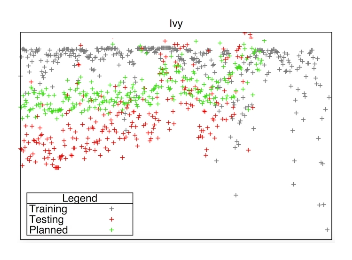
\includegraphics[width=\linewidth]{figs/2d.eps} 
		%  % 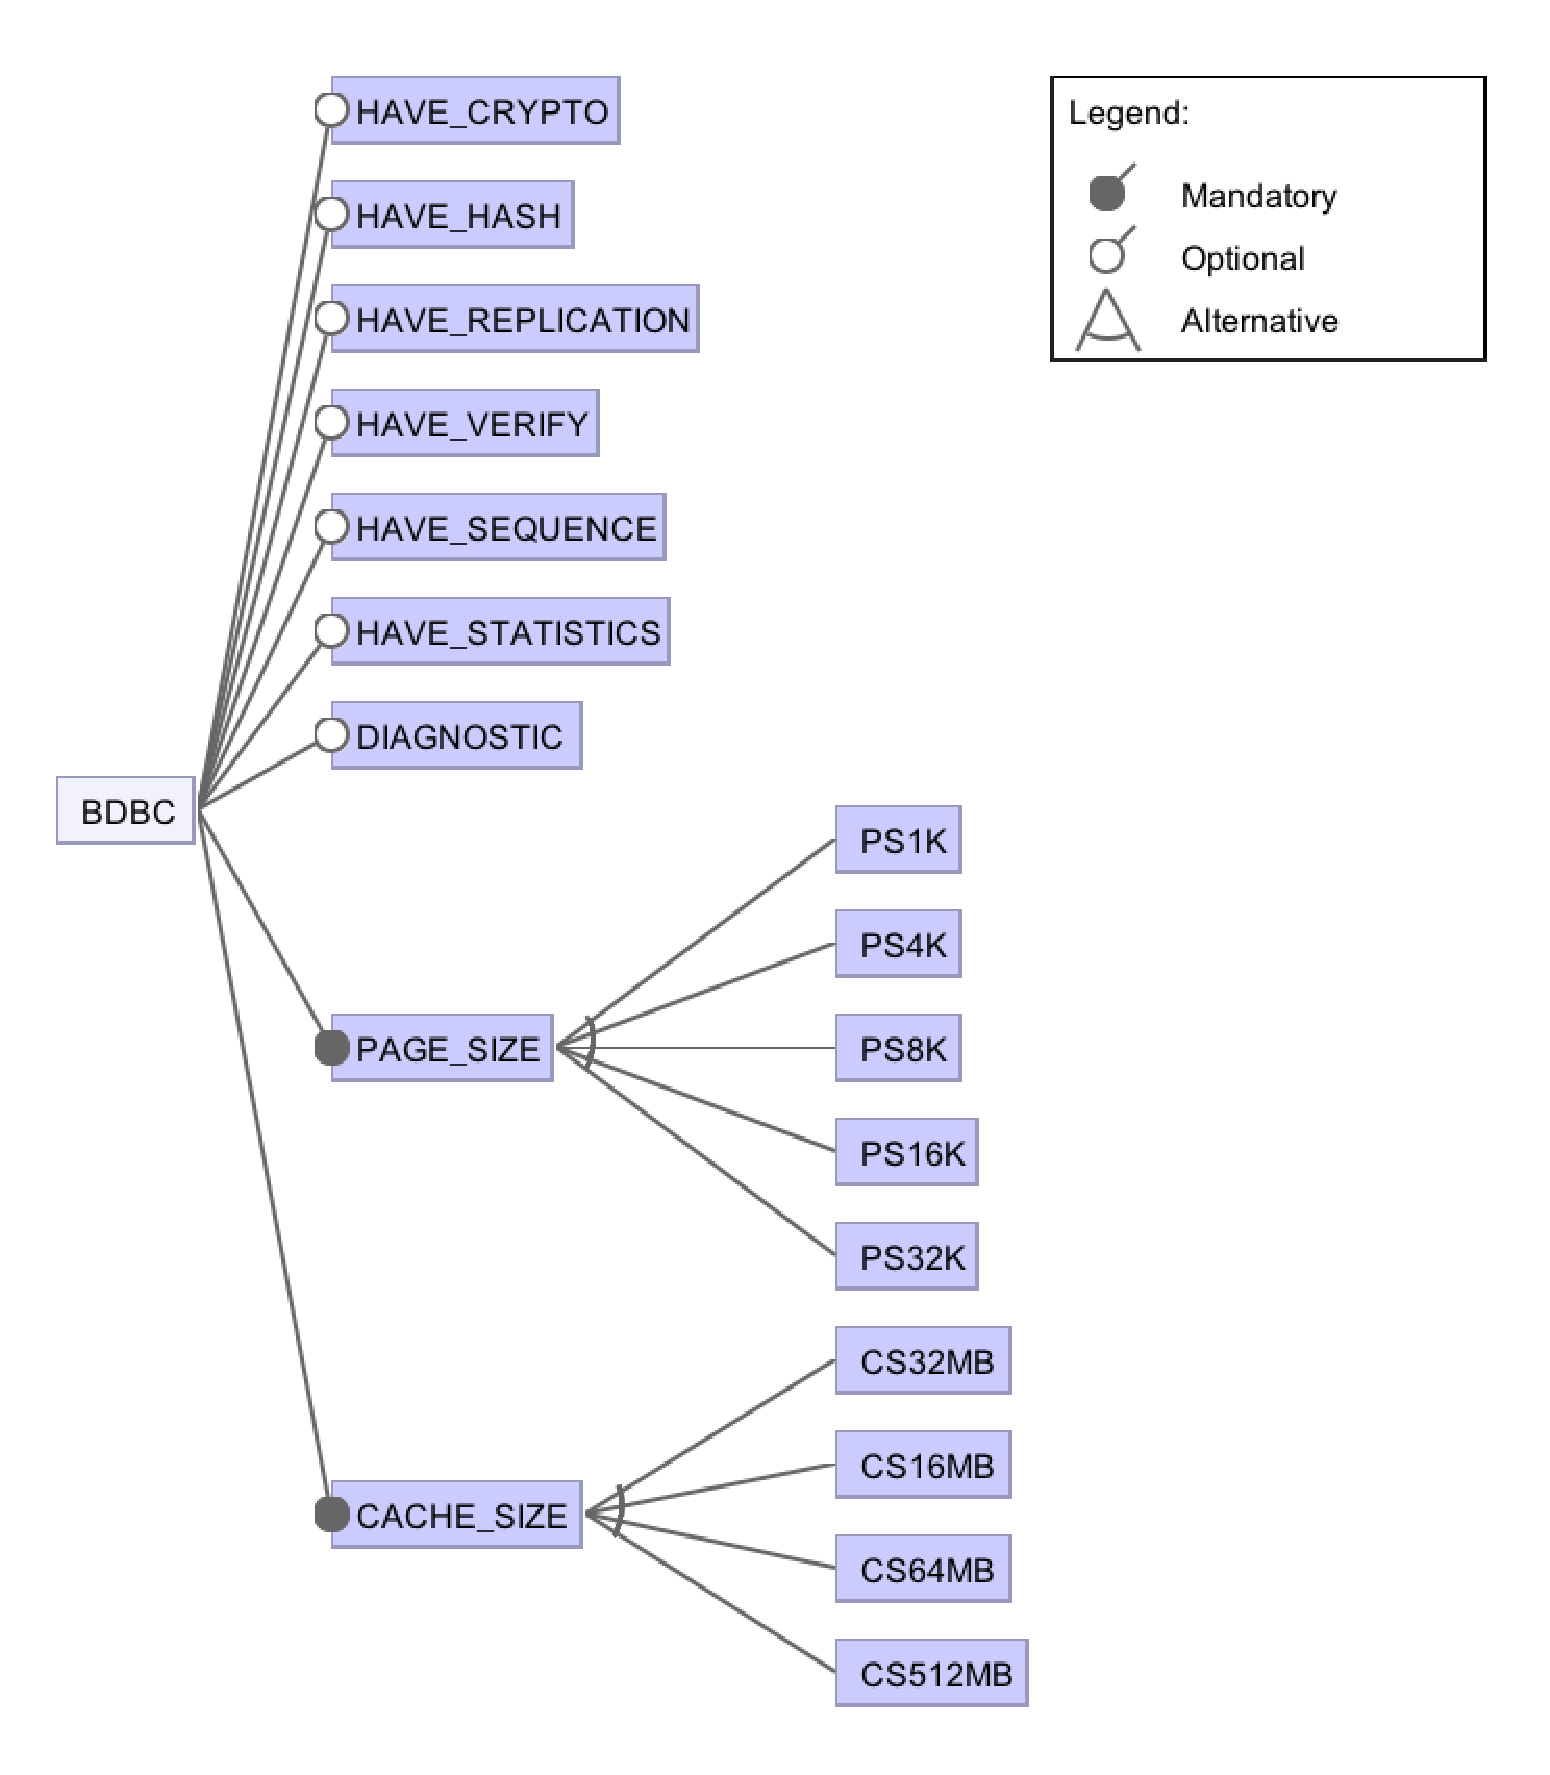
\includegraphics[width=1\linewidth]{figs/BDBC.eps}
		% \caption{Gray, red, green show (1) training examples, (2) test examples and 
		%   (3) tests that have been altered by planners.
		%   This figure uses axes generated from the first two components of a PCA analysis of all points. 
		% }\label{fig:howxy}
		% \end{figure}
		% We should mistrust the predictions made by a  model   if it is being applied to examples  that are
		% too far away from the
		% training cloud.
		% To test for ``too far'', we can run a data mining experiment that tests how well
		% a model learned from the training data applies to the test data. Such experiments return some performance value.
		
		% Note that predictions  about changes that  fall within the space of the training+test data, will be at least
		% as accurate as the predictions of the original test data. With this, we assert that the predictions for changes that move examples towards/away from the training data can be trusted more/less (respectively).
		
		% Accordingly, we need {\em trust-increasing} planners to generate new examples {\em closer} to the
		% training examples.  To see how this works, 
		%  \fig{howxy} is from the {\em ivy} data
		% set (one of the Jureczko data sets used in this paper). It shows: (1)~the training examples in gray, (2)~the test examples in red, and (3)~the
		% changed  examples displaced after applying a plan (in green).
		%  Note that the  the   changed examples
		% cases  (shown in green)  fall closer to the training cases (shown in gray) than
		% the test cases (shown in red). 
		
		% In that green region of changed examples, our belief in the value of predictions
		% will be just as much as, if not more than, our belief in the value of the predictions in the red region (that
		% contains the original test data).
		% This pattern of \fig{howxy} (where the new examples are found closer to  the training cases than the test cases) has been observed in all the other data sets studied in this
		% paper. Hence,  we can assert that
		% predictors learned from these training examples have some authority in the regions
		% containing the changes examples.
		
		
		% That said, the above comes with some important caveats:
		% \bi
		% \item 
		% The quality of the prediction depends on the nature of the training data. Thus, we strongly recommend that both the data set and the predictor be assessed prior to planning. This ensures that the predictor's performance is adequate for a data set. We tackle this issue in detail in \tion{tesd}.
		% \item
		% Planners should be designed to be {\em trust increasing}. We list four such planning methods in \tion{planners}.
		% \item
		% Where possible, planners should be assessed via some external
		% oracle that can accurately assess new examples. For an example of that kind of analysis,
		% see  \tion{coc}.
		% \ei
		
		% \subsection{  Internal Validity}\label{sect:coc}
		
		% % The main internal validity threat   in this study was the use of
		% % optimistic reasoning when generating the changed code modules.
		% We assumed in \tion{rq}
		% that any code module can be changed in order
		% to discourage triggering a bad smell detector. This is not necessarily
		% true, as noted in {\em PROBLEM \#2} in this paper's introduction.
		% To mitigate this issue:
		% \begin{itemize}
		%     \item We do not propose using XTREE as a bad
		% smell generator;
		% \item Rather, we offer it as  a critique agent for bad smells
		% proposed by some other oracle (e.g. a human developer).
		% \end{itemize}
		% We showed about that XTREE's recommendations are not verbose.
		% That is, even if XTREE recommends the superset of possibly important bad smells,
		% that superset is not so large as to  overlap with many
		%  bad smell proposed at random 
		% by   developers. 
		
		% XTREE does not require a working defect predictor to generate
		% its bad smell thresholds. However, to {\em certify}
		% that those thresholds are satisfactory, some
		% second quality predictor must be applied. A data set containing defect counts before and after refactoring activities would enable an accurate assessment of the performance of the threshold-setting and recommender methods, however, such a data set is not available at this time.
		
		%  Historically,
		% SE researchers~\cite{Cheng10,OKeeffe08,OKeeffe07,Moghadam2011,Mkaouer14} have used the QMOOD hierarchical quality model~\cite{Bansiya02}.
		% Since such quality models may be very project specific~\cite{localvsglobal}, we prefer building local 
		% defect predictors using Random Forests. We chose this approach,  based on its reputation for having the better  performance of 21 other learners for defect prediction~\cite{lessmann}.  
		% Our results show that when a defect log contains too few
		% non-defective examples then defector predictors
		% perform poorly (see the data sets in the last few lines of \fig{j})
		% as do their associated bad smell threshold generators
		% (recall the performance of Lucene and Poi in~\fig{jur}). It should be noted that this is not a limitation of XTREE-- rather
		% it seems fundamental to the problem of certifying bad smells.
		% As evidence of this, recall that {\em all} the bad smell threshold generators of~\fig{jur}
		% had issues with the defect data sets with  many defects
		% (Lucene and Poi).
		
		
		% % \subsection{ Learner Bias}
		% % This study used two kinds of learners: (1) methods for suggesting
		% % changes to code like Shatnawi, Alves et al., CD and XTREE;
		% % (2) methods for assessing the changes proposed by these learners.
		% % Prior studies implemented (2) using  the QMOOD hierarchical quality model
		% % which is so old, that we suspect it may no longer be current. Hence,
		% % we used Random Forests to build the assessment oracles that were specific
		% % to the data sets used in this study. We chose this approach,  based on its reputation for having the better  performance of 21 other learners for defect prediction~\cite{lessmann}. 
		
		
		
		
		
		% % \subsection{  Sampling bias} 
		% % Sampling bias threatens any data mining experiment; i.e., what matters
		% % there may not be true here. For example, the data sets used here comes from two  Jureczko et al. and any biases in their selection procedures
		% % threaten the validity of these results. 
		% % That said,
		% % the best we can do is define our methods and publicize our data and code so that other researchers can
		% % try to repeat our results and, perhaps, point out a previously unknown bias
		% % in our analysis. Hopefully, other researchers will emulate our methods in
		% % order to repeat, refute, or improve our results. 
		
		
		
		
		
		% \begin{figure}[!t]
%\noindent\begin{minipage}{0.5\textwidth} 
{\small 
\begin{tabular}{llrrc}
\arrayrulecolor{lightgray}
\rowcolor{lightgray}\textbf{Rank} & \textbf{Treatment} & \textbf{Median} & \textbf{IQR} & \\\hline
  1 &        XTREE &   59   &  9 & \quart{75}{4}{78}{99} \\
2 &      CD &    -9  &  77 & \quart{21}{41}{42}{99} \\
\hline \end{tabular}}
\caption{Planners applied to some ground-truth data (in this case, the POM3 model).
Values collected from  40 repeated runs of each method with different random seeds.
Results show the efficacy of XTREE in reducing the total overall cost in the original test data, when CD fail to do so.}
\label{fig:coc}
\end{figure}
		
		
		\section{Conclusions}
		How to discourage useless refactorings?
		We say: ignore those not supported by the historical log of data from
		the current project.  
		When that data is not available (e.g. early
		in the project) then developers could use the general list of
		bad smells shown in \fig{smells}. However, 
		our results
		show that  bad smell detectors are most
		effective when they are based
		on a small handful of code metrics (as done by XTREE).
		Hence, using all the bad smells of \fig{smells} may not be optimal. 
		
		For our better guess at how to reduce defects by changing code attributes,
		see  Figure ~\ref{fig:multcomp}. But given the large variance if the change recommendations, we strongly advice teams to use
		XTREE on their data to find their own best local changes.
		
		XTREE improves on prior methods for generating bad smells:
		\begin{itemize}
			\item As described in \tion{prelim}, bad smells generated by humans may not be applicable to the current project. On the other hand, XTREE can automatically learn specific thresholds
			for bad smells for the current project.
			\item Prior methods used an old quality predictor (QMOOD) which we replace with defect predictors learned via Random Forests
			from   current project data.
			
			
			\item XTREE's conjunctions proved to be arguably as effective
			as those of Alves (see \fig{jur}) but far less verbose (see \fig{counts}). Since XTREE {\em approves} of fewer changes
			it hence {\em disapproves} of most changes. This makes it a better tool for critiquing and rejecting
			many of the refactorings.
		\end{itemize}
		Finally, XTREE does not suffer from the conjunctive fallacy.
		Older methods, such as those proposed by  Shatnawi and Alves assumed
		that the best way to improve code is to remove outlier  values. This may not work since when code is refactored,
		{\em the functionality has to go somewhere}. Hence,  reducing the lines of code in one module necessitates   
		{\em increasing} the coupling that module
		to other parts of the code. In future, we recommend software team use bad smell detectors that know what attribute measures
		need {\em decreasing} as well as {\em increasing}.
		
		% In summary, this paper offers a baseline result
		% that XTREE can be used as a {\em diagnostic tool}
		% for identifying which bad smells can be ignored.
		% Can it be used as a {\em prescriptive tool}
		% to recommend new refactorings? This would require
		
		% As discussed in {\em PROBLEM \#2}
		% (from the introduction), XTREE might propose
		% changes to code metrics that are
		% not feasible  (due to the local domain constraints
		% of the code). To repair this, XTREE needs to be extended
		% with architectural knowledge of the code it is studying.
		% Elsewhere, we have had some   success
		% with reasoning about such architectural knowledge
		% (expressed as software product lines~\cite{sayyad13a,sayyad13b}). In future
		% work, we will explore extending XTREE 
		% with  
		% architectural knowledge such that it can
		% become a tool which perscribes
		% feasible refactorings. 
		
		
		\section*{Acknowledgements}
		The work is partially funded by NSF  awards \#1506586 and \#1302169.
		
		% \bibliographystyle{plain}
		\balance
		\bibliographystyle{unsrt}
		\bibliography{References}
	\end{document}